%chapters/3-deep-computations/

\chapter{Deep Computations}\label{ch:deep_computations}

The contents of this chapter are based on the author's contributions to and perspectives on our article~\cite{Duenezetal2026}, the second paper in a series started by the authors of \cite{alva2024approximability} that connects model theory, structural Ramsey theory, and the topology of function spaces to the foundational study of ``deep computations.''
While the initial work in \cite{alva2024approximability} established the formal framework for ultracomputations, characterizing them as accumulation points of standard computations and proving the existence of deep equilibria, this chapter focuses on the complexity and classification of this asymptotic behaviour.

Within the thesis, this chapter sits between the descriptive combinatorics of Chapter~\ref{ch:descriptive_combinatorics} and the Polish group actions of Chapter~\ref{ch:group_actions}, and the unifying thread is descriptive set theory at successive levels of the Baire-class hierarchy: Chapter~\ref{ch:descriptive_combinatorics} works at the Borel level, while this chapter works one step higher, with compact subsets of the first Baire class.
The dichotomy-and-basis paradigm developed in Chapter~\ref{ch:descriptive_combinatorics}, where definability has a structural cost, and the obstructions form a small canonical library, recurs here in a new way: the obstructions are now the seven prototype Rosenthal compacta of Argyros--Dodos--Kanellopoulos, and the cost is paid in approximability.
Rosenthal's dichotomy (Theorem~\ref{thm:Rosenthal} of Chapter~\ref{ch:introduction}) is the seed of this development.

% /chapters/3-deep-computations/01-intro.tex

\section{Introduction}\label{sec:deep_comp_intro}

In this chapter we study the asymptotic behavior of computations as parameters of the computation tend towards a limit, e.g., the depth of a neural network tending to infinity, or the time interval between layers of a time-series network tending toward zero.
Recently, particular cases of this concept have attracted considerable attention in deep learning research (e.g., Neural Ordinary Differential Equations~\cite{Chen:2018}, Physics-Informed Neural Networks~\cite{Raissi-Perdikaris-Karniadakis:2019}, and Deep Equilibrium Models~\cite{Bai:2019}).
The formal framework introduced here provides a unified setting to study these limit phenomena from a foundational viewpoint.

The main result of the chapter is the identification of a hierarchy of four distinct complexity classes for limit computations.
This is obtained by invoking a major result about the topology of spaces of functions, namely,
Todorčević's trichotomy for Rosenthal compacta~\cite{Todorcevic_1999_CompactSubsetsBaire} and transferring it into the realm of computation.
The medium that we use to translate between topology and computation is model theory, specifically, Shelah's classification theory~\cite{Shelah:1990}.

The translation between topology and computation proceeds as follows.
To every computation in a given computation model, we associate a continuous real-valued function, called the \emph{type} of the computation, that describes the logical properties of this computation with respect to the rest of the model.
This association allows us to view computations in any given computational model as elements of a space of real-valued functions, which is called the \emph{space of types} of the model.
The idea of embedding models of theories into their type spaces is borrowed from model theory, where type spaces play a central role.
The embedding of computations into spaces of types then allows us to utilize the vast theory of topology of function spaces, known as \emph{$\Cp$-theory}, to obtain results about complexity of topological limits of computations.
As we shall indicate next, recent classification results for spaces of functions provide an elegant and powerful machinery to classify computations according to their levels of ``tameness'' or ``wildness'', with the former corresponding roughly to polynomial approximability and the latter to exponential approximability.
The model-theoretic viewpoint of spaces of types thus allows us to interconnect various classification programs: 
in topology, the classification of Rosenthal compacta pioneered by Todorčević~\cite{Todorcevic_1999_CompactSubsetsBaire}; 
in logic, the classification of theories developed by Shelah~\cite{Shelah:1990}; and in statistical learning, the notions of PAC learning and VC dimension pioneered by Vapnik and Chervonenkis~\cite{Vapnik-Chervonenkis:1974, Vapnik-Chervonenkis:1971}.

In~\cite{alva2024approximability}, the authors introduced the concept of limits of computations, which they called \emph{ultracomputations} (given that they arise as ultrafilter limits of standard computations) and \emph{deep computations} (following usage in machine learning~\cite{Bai:2019}).
There is a technical difference between both designations, but in this chapter, to simplify the nomenclature, we will ignore the difference and use primarily the term ``deep computation''.

In \cite{alva2024approximability}, a new ``tame vs.\ wild'' (i.e., polynomially approximable vs.\ nonpolynomially approximable) dichotomy for the complexity of deep computations was proved by invoking a classical result of Grothendieck from the 1950s~\cite{Grothendieck:1952}.
Under our model-theoretic framework, the property of polynomial approximability of computations is identified with continuous extensibility in the sense of topology, and with the notions of \emph{stability} and \emph{type definability} in the sense of model theory.

In this chapter, we refine the dichotomy of \cite{alva2024approximability}, and obtain new complexity classes for deep computation.
The ``wild'' part of the dichotomy from~\cite{alva2024approximability} is further subdivided between ``tame'' and ``wild'' classes; three new levels of tameness are identified within this new subdivision, and seven distinct minimal prototypes of tameness are identified.

The finer classification results of this chapter are obtained through more contemporary topological and model-theoretic tools than in~\cite{alva2024approximability}. 
From the topological side, instead of Grothendieck's classical criterion, we use the modern theory of \emph{Rosenthal compacta}, and from the model theory side, instead of stability, we use \emph{neostability}.
The main tool imported from neostability is Shelah's \emph{Independence Property}, or rather, its negation, which is commonly referred to as ``NIP''.
More on this below.

Deep computations arise as topological limits of standard (continuous) computations.
In topology, the \emph{first Baire class}, or \emph{Baire class~1} consists of functions (also called simply \emph{Baire-1}) arising as pointwise limits of sequences of continuous functions.
Intuitively, the first Baire class consists of functions with ``controlled'' discontinuities, and lies just one level of topological complexity above the Baire class 0, which (by definition) consists of continuous functions.

We apply a result of Bourgain, Fremlin and Talagrand from the late 1970s on compact subsets of the first Baire class to obtain a new ``tame vs.\ wild'' dichotomy for deep computations~\cite{BFT_1978_PCompactBaire}; then, we apply a trichotomy of Todorčević, from the late 90s, for \emph{Rosenthal compacta} to identify new tame classes~\cite{Todorcevic_1999_CompactSubsetsBaire}.

A Rosenthal compactum is a compact topological space that is homeomorphic to a subspace of the space of Baire class~1 functions on some Polish (i.e., separable, completely metrizable) space equipped with the topology of pointwise convergence.
Rosenthal compacta exhibit ``topological tameness,'' meaning that they behave in relatively controlled ways.
Since the late 1970s, they have played a crucial role in understanding the complexity of structures of functional analysis, especially Banach spaces.
Todorčević's trichotomy for Rosenthal compacta has been utilized to settle longstanding problems in topological dynamics and topological entropy~\cite{glasner2022tame}.
It is noteworthy that Todorčević's proof relies on sophisticated set-theoretic forcing and infinite Ramsey theory.
At the time of writing this chapter, decades after his original argument, there are no elementary proofs of the trichotomy; in fact, Todorčević's methods have been analyzed and exploited further~\cite{Todorcevic:2023,horowitz2019compactsetsbaireclass}.
(Theorem~\ref{thm:Rosenthal} of Chapter~\ref{ch:introduction} is the prototype: a pointwise-bounded sequence in $\overline{\Cp(X)}$ either has a convergent subsequence or has $\beta\mathbb{N}$ as its pointwise closure: the simplest tame/wild split.)

Through our framework, Rosenthal compacta in topology correspond to the important concept of \emph{Non-Independence Property} (known as ``NIP'') in model theory, identified by Shelah~\cite{Shelah:1971,Shelah:1990}, and to the concepts \emph{VC-dimension} and \emph{Probably Approximately Correct} learning (known as ``PAC learnability'') in statistical learning theory~\cite{Vapnik-Chervonenkis:1971, Vapnik-Chervonenkis:1974, Valiant:1984}.

Beyond Todorčević's trichotomy, we invoke a more recent heptachotomy for separable Rosenthal compacta obtained by Argyros, Dodos and Kanellopoulos~\cite{argyros2008rosenthal}.
These authors identify seven fundamental ``prototypes" of separable Rosenthal compacta, and show that any non-metrizable separable Rosenthal compactum must contain a ``canonical'' embedding of one of these prototypes.

From the point of view of approximation theory, it is noteworthy that in the context of Gro\-then\-dieck~\cite{Grothendieck:1952} and Bourgain--Fremlin--Talagrand~\cite{BFT_1978_PCompactBaire}, compactness and sequential compactness coincide; thus, the results of these papers allow us to ensure that deep computations, which in principle are abstract ultrafilter limits (over a possibly uncountable set), can always be approximated by concrete \emph{sequences} of standard computations.

We believe that the results presented in this chapter show practitioners of computation, or topology, or descriptive set theory, or model theory, how classification invariants used in their field translate into classification invariants of other fields.
In the interest of accessibility, we do not assume that the reader has previous familiarity with advanced topology, model theory, or computing.
The necessary topological background beyond undergraduate topology is covered later in this section.

In this section, we also present basic topological and combinatorial preliminaries. In section~\ref{sec:CCS}, we introduce the structural/model-theoretic viewpoint (no previous exposure to model theory is needed).
Section~\ref{sec:classification} is devoted to the classification of deep computations.

Throughout the chapter, our results pertain to classical models of computation (particularly computations involving real-valued quantities that are known and manipulated to a finite degree of precision).
The final section, Section~\ref{sec:measure-theoretic-NIP}, introduces a probabilistic viewpoint, which we intend to develop in future work.

In this section we recall notions and results from general topology and function space theory.
For simplicity, we assume that all spaces are Hausdorff unless explicitly stated otherwise.

A subset of a topological space is $F_\sigma$ if it is a countable union of closed sets, and $G_\delta$ if it is a countable intersection of open sets.
In a metric space, every open set is~$F_\sigma$; equivalently, every closed set is~$G_\delta$.

A \emph{Polish space} is a separable and completely metrizable topological space, i.e., one admitting a complete metric that induces its topology.
The class of Polish spaces is closed under countable topological products.
Classical examples of Polish spaces (besides the real line) include the Cantor space~$2^\mathbb{N}$ (the set of all infinite binary sequences, endowed with the product topology), the Baire space $\mathbb{N}^\mathbb{N}$ (the set of all infinite sequences of naturals, also with the product topology), and the space $\mathbb{R}^\mathbb{N}$ of sequences of real numbers.

\begin{fact}\cite[4.3.24]{Engelking:1989}
A subset of a Polish space is itself Polish in the subspace topology if and only if it is a $G_{\delta }$ set.
In particular, closed subsets and open subsets of Polish spaces are also Polish spaces.
\end{fact}

If $X$ is a topological space and $A$ is a subset of $X$, then $A$ is said to be
\emph{nowhere dense} if its closure has an empty interior,
and of the \emph{first category} if $A$ is a countable union of closed nowhere dense sets;
otherwise, $A$ is said to be of the \emph{second category}.
Sets $A\subseteq X$ of the first category are also called \emph{meagre}, and their
complements $X\setminus A$ are called \emph{comeagre}.
Thus, the set of meagre subsets of $X$ is the $\sigma$-ideal generated by the nowhere dense subsets of $X$.
A topological space $X$ is \emph{Baire} if every comeagre subset of $X$ is dense.
Equivalently, $X$ is Baire if any countable intersection of open dense sets remains dense.
The Baire Category Theorem states that compact Hausdorff spaces and all completely metrizable spaces (hence, all Polish spaces) are Baire.%
\footnote{More generally, any Čech-complete space is Baire~\cite[Theorem 3.9.3]{Engelking:1989}.}

Given two topological spaces $X$ and $Y$ we denote by $\Cp(X,Y)$ the set of all continuous functions $f\colon X\rightarrow Y$ endowed with the topology of pointwise convergence, i.e., with the relative (subspace) product topology~$\Cp(X,Y)\subseteq Y^X$, where the product topology on $Y^X$ uses only $Y$'s topology; the topology on $X$ enters through the requirement that elements of $\Cp(X,Y)$ be continuous.
The space $\Cp(X, \mathbb{R})$ of continuous real-valued functions on~$X$ is denoted simply~$\Cp(X)$.

A function $f\in Y^X$ between topological spaces $X$, $Y$ is said to be of \emph{Baire class~1}, or a \emph{Baire-1} function, if there is a sequence $(f_n)_{n\in \mathbb{N}}\subseteq \Cp(X, Y)$ such that $f = \lim_{n\to\infty}f_n$ (i.e., $f(x)=\lim_{n\to\infty}f_n(x)$ for all $x\in X$).
An elementary argument shows that Baire-1 functions are continuous everywhere except on a set of the first category.
If $X$ and $Y$ are topological spaces, the space of Baire-1 functions $f\colon X\rightarrow Y$ endowed with the topology of pointwise convergence is denoted $\mathrm{B}_1(X,Y)$;
thus, $\Cp(X,Y)\subseteq \mathrm{B}_1(X,Y)\subseteq Y^X$ are topological inclusions.
We abbreviate $\mathrm{B}_1(X, \mathbb{R})$ as $\mathrm{B}_1(X)$.
Relatively compact subsets of $\Cp(X)$ and of $\mathrm{B}_1(X)$ (particularly for $X$ Polish) are of interest in analysis and topological dynamics.

A topological space $X$ is \emph{perfectly normal} if it is normal and every closed subset of $X$ is a $G_\delta$ set (equivalently, every open subset of $X$ is an $F_\sigma$ set).
Every metrizable space (hence, every Polish space) is perfectly normal.

The following fact was proved by Baire in his groundbreaking thesis.
For a proof, see~\cite[Section 10]{Todorcevic_1997_TopicsTop}.

\begin{fact}[Baire]\label{baire}
    If $X$ is perfectly normal, then the following conditions are equivalent for a function $f\colon X\to \mathbb{R}$:
    \begin{itemize}
        \item[(1)] $f$ is a Baire class~1 function, that is, $f$ is a pointwise limit of continuous functions.
        \item[(2)] $f^{-1}[U]$ is an $F_\sigma$ subset of $X$ whenever $U\subseteq\mathbb{R}$ is open.
    \end{itemize}
    If $X$ is Baire, then (1) and (2) are equivalent to:
    \begin{itemize}
        \item[(3)] For every closed $F\subseteq X$, the restriction $f|_F$ has a point of continuity.
    \end{itemize}
    Moreover, if $X$ is Polish and $f\notin \mathrm{B}_1(X)$, then there exist countable $D_0,D_1\subseteq X$ and reals $a<b$ such that
    \[
    D_0\subseteq f^{-1}(-\infty,a],
    \quad
    D_1\subseteq f^{-1}[b,\infty),
    \quad
    \overline{D_0}=\overline{D_1}.
    \]
\end{fact}

\subsection{From Rosenthal's dichotomy to the Bourgain--Fremlin--Talagrand dichotomy to Shelah's NIP}

Recall the following result from the Introduction chapter.

\rosenthaldichotomy*

The genesis of the dichotomy was \emph{Rosenthal's $\ell_1$-Theorem}, which states that a Banach space includes an isomorphic copy of $\ell_1$ (the space of absolutely summable sequences), or else every bounded sequence therein is weakly Cauchy.
The $\ell_1$-Theorem connects diverse areas:
Banach space geometry, Ramsey theory, set theory, and topology of function spaces.

As we move from $\Cp(X)$ to the larger space $\mathrm{B}_1(X)$, a dichotomy paralleling the $\ell_1$-Theorem holds.
This result is usually not phrased as a dichotomy in the above manner, but rather as an equivalence (see Theorem~\ref{thm:BFT} below).

First, we introduce some useful notation.
For any $f\in \mathbb{R}^X$ and any real $a$, define
\begin{align*}
    X^f_{\le a} &\coloneqq f^{-1}(-\infty,a], &
    X^f_{\ge a} &\coloneqq f^{-1}[a, +\infty).
\end{align*}
For any set $A\subseteq \mathbb{R}^X$ and any real $a$, define (by a slight abuse of notation)
\begin{align*}
    X^A_{\le a} &\coloneqq \bigcap_{f\in A}X^f_{\le a} = \{x\in X: \text{$f(x)\le a$ for all $f\in A$}\},\\
    X^A_{\ge a} &\coloneqq \bigcap_{f\in A}X^f_{\ge a} = \{x\in X: \text{$f(x)\ge a$ for all $f\in A$}\}.
\end{align*}
(In case $A=\emptyset$, we define $X^\emptyset_{\ge a} = X = X^\emptyset_{\le a}$.)
For any sequence $\{f_n\}\subseteq \mathbb{R}^X$ and $I\subseteq \mathbb{N}$, define $I^{\complement} \coloneqq \mathbb{N}\setminus I$ and $f_I \coloneqq \{f_i: i\in I\}$.

\begin{theorem}[``The BFT Dichotomy''. Bourgain--Fremlin--Talagrand {\cite{BFT_1978_PCompactBaire}}]
\label{thm:BFT}
    Let $X$ be a Polish space and $A\subseteq \Cp(X)$ be pointwise bounded.
    The following are equivalent:
    \begin{enumerate}[(i)]
        \item $A$ is relatively compact in $\mathrm{B}_1(X)$.
        \item For every $(f_n)_{n\in\mathbb{N}}\subseteq A$ and every $a<b$ there is $I\subseteq\mathbb{N}$ such that
        \begin{equation*}
            X_{\le a}^{f_I} \cap X_{\ge b}^{f_{I^{\complement}}} = \emptyset.
        \end{equation*}
    \end{enumerate}
\end{theorem}
(As stated above, the BFT Dichotomy is a particular case of the equivalence (ii)$\Leftrightarrow$(v) in {\cite[Corollary 4G]{BFT_1978_PCompactBaire}}.)

The sets $X_{\le a}^{f_I}$ and $X_{\ge b}^{f_{I^{\complement}}}$ appearing in condition Theorem~\ref{thm:BFT}\emph{(ii)} are defined, respectively, in terms of $|I|$-many inequalities of the form $f_i(x)\le a$, and $|I^{\complement}|$-many of the form $f_j(x)\ge b$.
Thus, at least one of $X_{\le a}^{f_I}$ and $X_{\ge b}^{f_{I^{\complement}}}$ is defined by the satisfaction of infinitely (countably) many inequalities.
For our purposes, it is more natural to consider only finitely many inequalities at a time, which motivates the definitions below.

\begin{definition}\label{def:NIP-fns}
    We say that a collection of functions \emph{$A\subseteq \mathbb{R}^X$ has the finitary Non-Independence Property (NIP)} if, for all sequences $(f_n)_{n\in\mathbb{N}}\subseteq A$ and reals $a<b$, there exist finite disjoint sets $E,F\subseteq\mathbb{N}$ such that $X_{\le a}^{f_E} \cap X_{\ge b}^{f_F} = \emptyset$.
    We say that such $E, F$ \emph{witness finitary NIP for $(f_n)$ and $a, b$}.

    A set $A\subseteq \mathbb{R}^X$ \emph{has the finitary Independence Property (IP)} if it does not have finitary NIP, i.e., if there exists a sequence $(f_n)_{n\in\mathbb{N}}\subseteq A$ and reals $a<b$ such that for every pair of finite disjoint sets $E,F\subseteq\mathbb{N}$, we have $X_{\le a}^{f_E} \cap X_{\ge b}^{f_F} \ne \emptyset$.
\end{definition}

If the word ``finite'' is omitted in the above definitions, we obtain the definitions of \emph{countable} NIP (weaker than finitary NIP) and \emph{countable} IP (stronger than finitary IP), respectively.

If we insist on witnesses $E,F\subseteq \mathbb{N}$ such that $F = E^{\complement}$, we call the respective properties ``BFT-NIP'' and ``BFT-IP''.
Thus, Theorem~\ref{thm:BFT} becomes (for pointwise bounded function collections $A\subseteq \Cp(X)$) that $A$ is relatively compact in $\mathrm{B}_1(X)$ if and only if $A$ has BFT-NIP.

Unless otherwise unspecified, IP/NIP shall mean \emph{finitary} IP/NIP henceforth.

\begin{proposition}\label{prop:BFT-finitary-cpct}
    If $X$ is compact and $A\subseteq \Cp(X)$, then $A$ has BFT-NIP if and only if it has finitary NIP.
\end{proposition}
(No pointwise boundedness is assumed of~$A$.)
\begin{proof}
    Trivially (as per the preceding discussion), finitary NIP implies BFT-NIP.
    Reciprocally, assume that $X$ is compact and $A\subseteq \Cp(X)$ has finitary IP.
    Fix a sequence $(f_n)\subseteq A$ and reals $a<b$ such that $X^{f_E}_{\le a}\cap X^{f_F}_{\ge b}\neq\emptyset$ for every finite disjoint $E,F\subseteq\mathbb{N}$.
    Fix $I\subseteq\mathbb{N}$.
    Since $(f_n)\subseteq A\subseteq \Cp(X)$ is a sequence of continuous functions, the collection $\mathcal{F}_I=\{X^{f_n}_{\le a}:n\in I\}\cup\{X^{f_m}_{\ge a}:m\in I^{\complement}\}$ consists of closed (non-empty) sets.
    Since all finite $E\subseteq I$ and $F\subseteq I^{\complement}$ witness finitary IP for $(f_n)$ and $a, b$, we see that the collection $\mathcal{F}_I$ has the finite intersection property.
    By compactness, $X^{f_I}_{\le a}\cap X^{f_{I^{\complement}}}_{\ge b} = \bigcap\mathcal{F}_I\neq\emptyset$.
\end{proof}

\begin{theorem}\label{thm:BFT2}
    Let $X$ be a compact metrizable (hence Polish) space.
    For every pointwise bounded $A\subseteq \Cp(X)$, the following properties are all equivalent:
    \begin{enumerate}[(i)]
        \item $A$ is relatively compact in~$\mathrm{B}_1(X)$;
        \item $A$ has BFT-NIP;
        \item $A$ has countable NIP;
        \item $A$ has finitary NIP.
    \end{enumerate}
\end{theorem}

(The equivalence \emph{(ii)}$\Leftrightarrow$\emph{(iv)} holds for arbitrary compact~$X$.
The equivalence \emph{(ii)}$\Leftrightarrow$\emph{(iii)}, for arbitrary~$X$.)

\begin{proof}
    Corollary of Theorem~\ref{thm:BFT} and Proposition~\ref{prop:BFT-finitary-cpct}.
\end{proof}

Theorem~\ref{thm:BFT2} may be stated as the following dichotomy (under the assumptions) for any compact metrizable~$X$:
either $A$ is relatively compact in~$\mathrm{B}_1(X)$, or $A$ has IP (in either sense).

The Independence Property was first isolated by Saharon Shelah in model theory as a dividing line between theories whose models are ``tame'' (corresponding to NIP) and theories whose models are ``wild" (corresponding to IP).
See~\cite[Definition 4.1]{Shelah:1971}, \cite{Shelah:1990}.
We will discuss this dividing line in more detail in the next section.

\subsection{NIP as a universal dividing line between polynomial and exponential complexity}

The particular case of the BFT dichotomy (Theorem~\ref{thm:BFT}) when $A$ consists of $\{0,1\}$-valued (i.e., $\{\text{Yes},\text{No}\}$-valued) strings was discovered independently, around 1971-1972 in many foundational contexts related to polynomial (``tame") vs.\ exponential (``wild'') complexity: In model theory, by Saharon Shelah~\cite{Shelah:1971}, \cite{Shelah:1990}, in combinatorics, by Norbert Sauer~\cite{Sauer:1972}, and Shelah~\cite{Shelah:1972}, \cite{Shelah:1990}, and in statistical learning, by Vladimir Vapnik and Alexey Chervonenkis~\cite{Vapnik-Chervonenkis:1971}, \cite{Vapnik-Chervonenkis:1974}.


\begin{description}

\item[In model theory]
Shelah's classification theory is a foundational program in mathematical logic devised to categorize first-order theories based on the complexity and structure of their models.
A theory $T$ is considered classifiable in Shelah's sense if the number of non-isomorphic models of $T$ of a given cardinality can be described by a bounded number of numerical invariants.
In contrast, a theory $T$ is unclassifiable if the number of models of $T$ of a given cardinality is the maximum possible number.
A key fact is that the number of models of $T$ is directly impacted by the number of \emph{types} over sets of parameters in models of $T$; a controlled number of types is a characteristic of a classifiable theory.


In Shelah's classification program~\cite{Shelah:1990}, theories \emph{without} the independence property (called NIP theories, or \emph{dependent} theories) have a well-behaved, ``tame" structure;
the number of types over a set of parameters of size $\kappa$ of such a theory is of polynomially or similar “slow" growth on~$\kappa$.

In contrast, theories with the Independence Property (called IP theories) are considered “intractable" or “wild”.
A theory with the Independence Property produces the maximum possible number of types over a set of parameters; for a set of parameters of cardinality $\kappa$, the theory will have $2^{2^{\kappa}}$-many distinct types.

\item[In combinatorics]
Sauer~\cite{Sauer:1972} and Shelah~\cite{Shelah:1972} proved the following independently:
Let $\mathscr{F}$ be a collection of subsets of some set $S$.
Either:
for every $n\in\mathbb{N}$ there is a set $A\subseteq S$ with $|A|=n$ such that $|\{S_i\cap A: i\in\mathbb{N}\}|=2^n$ ($\mathscr{F}$ is a collection having ``exponential complexity'');
or: there exists $N\in\mathbb{N}$ such that for every $A\subseteq S$ with $|A|\ge N$, one has
\[
|\{S_i\cap A: i\in\mathbb{N}\}| \le \sum_{i=0}^{N-1} \binom{|A|}{i}.
\]
($\mathscr{F}$ is a collection having ``polynomial complexity'').
Clearly, any collection $\mathscr{F}$ of subsets of a \emph{finite} set $S$ has polynomial complexity.
The ``polynomial'' name is justified:
indeed, for fixed $N>0$, as a function of the size $|A| = m > 0$, we have
\begin{equation*}
    \sum_{i=0}^{N-1} \binom{m}{i}
    \le \sum_{i=0}^{N-1}\frac{m^{i}}{i!}
    \le \left( \sum_{i=0}^{N-1}\frac{1}{i!} \right)\cdot m^{N-1}
    < e\cdot m^{N-1} = O \left( m^N \right).
\end{equation*}
(More precisely, the order of magnitude is $O(m^{N-1})$:
polynomial in $m$ for $N$ fixed.)

\item[In machine learning]
Readers familiar with statistical learning may recognize the Sauer-Shelah lemma as the dichotomy discovered and proved slightly earlier (1971) by Vapnik and Chervonenkis~\cite{Vapnik-Chervonenkis:1971, Vapnik-Chervonenkis:1974} to address uniform convergence in statistics.
The least integer $N$ given by the preceding paragraph, when it exists, is called the \emph{VC-dimension} of $\mathscr{F}$;
it is a core concept in machine learning.
If such an integer $N$ does not exist, we say that the VC-dimension of $\mathscr{F}$ is infinite.
The lemma provides upper bounds on the number of data points (sample size) needed to learn a concept class of known VC dimension~$d$ up to a given admissible error in the statistical sense.
The Fundamental Theorem of Statistical Learning states that a hypothesis class is PAC-learnable (PAC stands for ``Probably Approximately Correct'') if and only if its VC dimension is finite.
 
\end{description}
 
\subsection{Rosenthal compacta}
 
The universal classification implied by Theorem~\ref{thm:BFT}, as attested by the examples outlined in the preceding section, led to the following definition (by Gilles Godefroy~\cite{Godefroy:1980}):

\begin{definition}
\label{def:Rosenthal-compacta}
A Rosenthal compactum is any topological space realized as a compact subset of the space $\mathrm{B}_1(X) = \mathrm{B}_1(X, \mathbb{R})$ (equipped with the topology of pointwise convergence) of all real functions of the first Baire class on some Polish space~\(X\).
\end{definition}
A Rosenthal compactum~$K$ is necessarily Hausdorff since it is a topological subspace of the Hausdorff product space $\mathbb{R}^X$.

Rosenthal compacta possess significant topological and dynamical tameness properties, and play an important role in functional analysis, measure theory, dynamical systems, descriptive set theory, and model theory.
In this chapter, we use them to study deep computations.
% For this, we shall first focus on countable languages, which is the theme of the next subsection.

\subsection{The special case~\texorpdfstring{$\mathrm{B}_1(X,\mathbb{R}^\mathcal{P})$}{B\_1(X, R\textasciicircum P)} with~\texorpdfstring{$\mathcal{P}$}{P} countable}

Fix an arbitrary (at most) countable set~$\mathcal{P}$ whose elements $P\in \mathcal{P}$ will be called \emph{predicate symbols} or \emph{formal predicates}.
Our present goal is to characterize relatively compact subsets of $\mathrm{B}_1(X,\mathbb{R}^\mathcal{P})$, where $X$ is always assumed to be a perfectly normal space (typically a Polish space).

The set $\mathcal{P}$ shall be considered discrete whenever regarded as a topological space.
Since $$\Cp(X, \mathbb{R}^{\mathcal{P}})\subseteq \mathrm{B}_1(X, \mathbb{R}^{\mathcal{P}})\subseteq (\mathbb{R}^{\mathcal{P}})^X,$$ the ``ambient'' space $(\mathbb{R}^{\mathcal{P}})^X$ is quite relevant.
The product $X\times \mathcal{P}$ will be regarded as either a point set, or as a topological product depending on context.
We have natural homeomorphic identifications
\begin{equation*}
    (\mathbb{R}^{\mathcal{P}})^X \cong \mathbb{R}^{X\times \mathcal{P}} \cong (\mathbb{R}^X)^{\mathcal{P}},
\end{equation*}
given by
\begin{align*}
    \mathbb{R}^{X\times \mathcal{P}} \to (\mathbb{R}^{\mathcal{P}})^X: \varphi &\mapsto {\hat{}}\varphi \\
    \mathbb{R}^{X\times \mathcal{P}} \to (\mathbb{R}^X)^{\mathcal{P}}: \varphi &\mapsto \varphi{\,\hat{}},
\end{align*}
where 
\begin{align*}
    \hat{}\varphi(x)\coloneqq \varphi(x, \cdot)\in \mathbb{R}^{\mathcal{P}}, &&
    \varphi\,\hat{}(P)\coloneqq \varphi(\cdot, P) \in \mathbb{R}^X.
\end{align*}
Such identifications view $X$ and $\mathcal{P}$ as mere point sets (the topology of~$X$ in particular plays no role).

For $x\in X$, define the ``left projection'' map
\begin{equation*}
    \lambda_x\colon \mathbb{R}^{X\times\mathcal{P}}\to \mathbb{R}^{\mathcal{P}}: \varphi\mapsto \lambda_x(\varphi)\coloneqq \hat{}\varphi(x);
\end{equation*}

for $P\in \mathcal{P}$, the ``right projection'' map
\begin{equation*}
    \rho_P\colon \mathbb{R}^{X\times\mathcal{P}}\to \mathbb{R}^X: \varphi\mapsto \rho_P(\varphi)\coloneqq \varphi\,\hat{}(P).
\end{equation*}
For fixed $x\in X$ and $P\in \mathcal{P}$, we also have canonical projection maps
\begin{align*}
    \lambda_x\colon \mathbb{R}^X\to \mathbb{R}: f\mapsto f(x), &&
    \rho_P\colon \mathbb{R}^{\mathcal{P}}\to \mathbb{R}: f\mapsto f(P).
\end{align*}
When clear from context, rather than using the specific symbols (``$\lambda$'' for left,``$\rho$'' for right) to denote projections, we may use the generic symbol~``$\pi$'';
thus, $\pi_x$ may mean $\lambda_x$, and $\pi_P$ may mean $\rho_P$.

The Proposition below reduces the study of $\mathbb{R}^{\mathcal{P}}$-valued continuous or Baire-1 functions on~$X$ to the special case of real-valued ones.

\begin{proposition}\label{prop:Baire-identifications}
    The identification $(\mathbb{R}^{\mathcal{P}})^X \cong \mathbb{R}^{X\times \mathcal{P}} \cong (\mathbb{R}^X)^{\mathcal{P}}$ induces identifications
    \begin{align*}
        \Cp(X, \mathbb{R}^{\mathcal{P}}) \cong \Cp(X\times \mathcal{P}) \cong \Cp(X)^{\mathcal{P}}, &&
        \mathrm{B}_1(X, \mathbb{R}^{\mathcal{P}}) \cong \mathrm{B}_1(X\times \mathcal{P}) \cong \mathrm{B}_1(X)^{\mathcal{P}}.
    \end{align*}
\end{proposition}

(The cardinality of $\mathcal{P}$ plays no role.)

\begin{proof}
    The identification of $\Cp$-spaces follows trivially from the definition of topological product and the fact that $\mathcal{P}$ is discrete: a continuous map $X\to \mathbb{R}^{\mathcal{P}}$ is precisely a $\mathcal{P}$-indexed family of continuous functions $X\to \mathbb{R}$, and these correspond to continuous functions $X\times \mathcal{P}\to \mathbb{R}$.
    The identification of Baire-1 spaces follows immediately, since it is defined in terms of the purely topological notion of limit (in the ambient space) of sequences of continuous functions.
\end{proof}

Given $A\subseteq Y^X$ and $K\subseteq X$ we write $A|_K:=\{f|_K:f\in A\}$, i.e., the set of all restrictions of functions in $A$ to $K$.
The following Theorem is a slightly more general version of Theorem \ref{thm:BFT}.

\begin{theorem}\label{thm:Generalized-BFT}
    Assume that $\mathcal{P}$ is countable, $X$ is a Polish space, and $A\subseteq \Cp(X,\mathbb{R}^\mathcal{P})$ is pointwise bounded in the sense that $\pi_P\circ A$ ($\subseteq \Cp(X)$) is pointwise bounded for every $P\in\mathcal{P}$.
    The following are equivalent for every compact $K\subseteq X$:

    \begin{enumerate}[(i)]
        \item $A|_K$ is relatively compact in $\mathrm{B}_1(K,\mathbb{R}^\mathcal{P})$;
        \item $\pi_P\circ A|_K$ has NIP for every $P\in\mathcal{P}$.
    \end{enumerate}
\end{theorem}

\begin{proof}
    Compact subsets $K\subseteq X$ are closed, hence also Polish.
    Therefore, the asserted equivalence follows from Theorems~\ref{thm:BFT} and~\ref{prop:BFT-finitary-cpct}.
\end{proof}

We conclude this section with an elementary but important observation.

\begin{lemma}\label{lem:NIP-and-closure}
    Assume that $X$ is Hausdorff and that $A\subseteq \Cp(X)$.
    The following are equivalent for every $L\subseteq X$:
    \begin{enumerate}[(i)]
        \item
        $A_L$ satisfies the NIP;
        \item
        $A|_{\overline{L}}$ satisfies the NIP.
    \end{enumerate}
\end{lemma}

\begin{proof}
    The implication (i)$\Rightarrow$(i) is trivial.  To see the opposite implication, suppose that (ii) does not hold, and choose $\{f_n\}_{n\in\mathbb{N}}\subseteq A$ and $a<b$ such that for all finite disjoint $E,F\subseteq\mathbb{N}$,
    \[
	\overline{L}\cap\bigcap_{n\in E}f_n^{-1}(-\infty,a]\cap\bigcap_{n\in F}f_n^{-1}[b,\infty)\neq\emptyset.
    \]
    But then, for any $a',b'$ with $a<a'<b'<b$ and any finite disjoint $E,F\subseteq\mathbb{N}$, we can choose
    \[
	x\in\overline{L}\cap\bigcap_{n\in E}f_n^{-1}(-\infty,a')\cap\bigcap_{n\in F}f_n^{-1}(b',\infty),
    \]
    which, by the definition of closure, gives
    \[
	L\cap\bigcap_{n\in E}f_n^{-1}(-\infty,a']\cap\bigcap_{n\in F}f_n^{-1}[b',\infty)\neq\emptyset,
    \]
    contradicting (i).
\end{proof}

\subsection*{Historical remarks}
The Baire hierarchy of functions was introduced by René-Louis Baire in his 1899 doctoral thesis, \emph{Sur les fonctions de variables réelles}.
The field of $\Cp$-theory was pioneered by A.~V.~Arhangel'skiĭ and his students in the 1970s and 1980s~\cite{Arkhangelskii:1992}, and
it has found many applications in model theory and functional analysis.
For a recent survey, see~\cite{tkachuk2011cp}.
% /chapters/3-deep-computations/02-CCS.tex

\section{Compositional Computation Structures}\label{sec:CCS}

In this section, we connect function spaces with arbitrary-precision computations.
We start by summarizing some basic concepts from~\cite{alva2024approximability}.

\subsection{Computation States Structures}
\label{sec:CSS}

A \emph{computation states structure} is a pair $(L,\mathcal{P})$, where $L$ is a set whose elements we call \emph{states} and $\mathcal{P}$ is a collection of real-valued functions on $L$ that we call \emph{predicates}, also called \emph{features}.
For each $P\in \mathcal{P}$, we call the value $P(v)$ the $P$-th \emph{(observable) feature} of~$v$.

A \emph{transition} of a computation states structure $(L,\mathcal{P})$ is a map $f\colon L\to L$.

The \emph{type} of a state $v\in L$ is the indexed family%
\footnote{As in~§\ref{prop:Baire-identifications} above, we regard each predicate on $L$ as named by a specific formal label~$P$ (a \emph{predicate symbol}) which is given the semantic meaning of a \emph{bona fide} real function $P(\cdot)\colon v\mapsto P(v)$ (the predicate proper) in the computation states structure.
Such a formal symbol~$P$ becomes \emph{de facto} the name of an observable feature having the real value $P(v)$ at any state $v\in L$.
Whenever $\mathcal{P}$ is used as an index set (e.g., as in the topological product $\mathbb{R}^{\mathcal{P}}$ below), it is regarded as a set of formal symbols.
This syntactic vs.\ semantic abuse of nomenclature is commonplace in mathematics, but the model-theoretic framework requires contextual awareness of the distinction.
To disambiguate when necessary, we shall write $P(\cdot)$, implying the semantic meaning of a real function on~$L$, in contrast to~$P$, meant as a purely syntactic symbol.
Nevertheless, by a standard abuse of nomenclature in appropriate contexts, we may also treat $P$ as a function on states (i.e., take $P$ to mean $P(\cdot)$ proper).}
\[
\operatorname{tp}(v)= (P(v))_{P\in \mathcal{P}}\in\mathbb{R}^\mathcal{P}
\]
of its features.

Intuitively, $L$ is the set of states of a computation, and the predicates $P \in\mathcal{P}$ are primitives that are given and accepted as computable.
(I.e., each symbol $P\in \mathcal{P}$ denotes a function $P(\cdot)$ taken as a computational primitive on~$L$.)

We assume that each state $v\in L$ is uniquely characterized by its type $\operatorname{tp}(v)$, so we may identify $L$ with a topological subspace of~$\mathbb{R}^\mathcal{P}$ and topologized as such (i.e., $L$ is identified with its forward image~$\tp[L]\subseteq \mathbb{R}^{\mathcal{P}}$ under the type map).
As a topological space, $L$ is thus endowed with the topology of pointwise convergence induced by the product topology of~$\mathbb{R}^\mathcal{P}$.
In particular, for each $P\in \mathcal{P}$, the projection map $v\mapsto P(v)$ is continuous.

Important state spaces include $L=\mathbb{R}^\mathbb{N}$ (resp., $L=\mathbb{R}^n$ for some positive integer~$n$), endowed with one predicate $P_i(v) = v_i$ (giving the $i$-th coordinate of~$v$) for each~$i\in \mathbb{N}$ (resp., for each $0\le i<n$).
State subspaces $L\subseteq \mathbb{R}^{\mathbb{N}}$ and $L\subseteq \mathbb{R}^n$ are of primary interest in this paper.
(Any states structure having a finite or countable family of predicates is effectively such a subspace.)

\begin{definition}
Given a computation states structure $(L,\mathcal{P})$, any type $\tp(v)\in \mathbb{R}^{\mathcal{P}}$ of a state $v\in L$ will be called a \emph{realized} (state) type.
The topological closure of the set of realized types in~$\mathbb{R}^\mathcal{P}$ (endowed with the pointwise convergence topology) will be called the \emph{space of (state) types} of~$(L,\mathcal{P})$, denoted~$\mathcal{L}$;
elements $\mathbf{v}\in \mathcal{L}$ are called \emph{state types}.
Elements $\mathbf{v}\in\mathcal{L}\setminus L$ are \emph{unrealized} state types.
\end{definition}

Intuitively, state types capture a notion of ``limit state''.
For each $P\in \mathcal{P}$, the $P$-th coordinate map (natural projection) $\mathbb{R}^{\mathcal{P}}\to \mathbb{R}: \mathbf{v} = (\mathbf{v}_Q)_{Q\in \mathcal{P}}\mapsto \mathbf{v}_P$, gives a continuous extension to~$\mathcal{L}$ of the predicate $P(\cdot)$ on~$L$;
abusing notation, the extension will still be denoted~$P(\cdot)$ (or just~$P$).

\begin{remark}\label{rem:poor-mans-ultraprod}
    Just as $L$ is identified with a subset of~$\mathcal{L}$, but going in the opposite direction, one may regard unrealized state types as “hyper-states” (when such type is obtained as a sequential limit—or ultralimit—of realized state types, unrealized state types may be called “deep states”).
    A comment for readers versed in model theory: at least for the purpose of realizing state types (with parameters in the original states space~$L$), the type space $(\mathcal{L}, \mathcal{P})$ serves as a “poor man's” ultraproduct of~$(L, \mathcal{P})$ wherein, by the very definition of~$\mathcal{L}$, each type $\mathbf{v}$ is realized.
\end{remark}

\subsubsection{Bounds on precision and magnitude. Shards}
\label{sec:shards}

In order for computation state structures to serve their purpose as models of real-world computing, we must keep in mind that computations involving real-valued quantities can only ever carried out approximately, to a preset degree of precision (i.e., to within acceptable error bounds).
More subtly, yet equally important in practice, one must also bound the magnitude of real quantities involved in all computations:
one cannot possibly store—let alone compute with—arbitrarily large numbers!
Thus, although the collection~$\mathcal{P}$ of predicates may be infinite (possibly, uncountable even), “true” computations must imply choices, at the outset, of bounds for errors and for absolute magnitudes of quantities involved.
Heuristically, different parts of a computation may require suitably matching (different) error bounds, as well as dealing with quantities of very different sizes.
Focusing for now on the second of these issues, our results shall generally apply to sets of computations for which arbitrary but fixed bounds for each predicate are set in advance.
This leads to the concept of \emph{shard} first introduced in~\cite{alva2024approximability}, as per the following definition.

\begin{definition}
    Fix a computation states structure $\underline{L} = (L, \mathcal{P})$, with $L\subseteq \mathbb{R}^{\mathcal{P}}$ implicitly identified with its type space.
    A \emph{sizer} is a family $r_{\bullet}=(r_P)_{P\in\mathcal{P}}$ of positive real numbers, indexed by~$\mathcal{P}$.
    Given a sizer $r_\bullet$, let $\mathbb{R}[\rb] \coloneqq \prod_{P\in\mathcal{P}}[-r_P,r_P]$ (a compact space), and let the $r_\bullet$-\emph{shard} of the states space~$L$ be $$L[r_\bullet] = L\cap \mathbb{R}[\rb].$$

For a sizer $r_{\bullet}$, the \emph{$r_{\bullet}$-type shard} is defined as $\mathcal{L}[r_\bullet]=\overline{L[r_\bullet]}$
(a closed, hence compact subset of $\mathbb{R}[\rb]$).

Let also $\mathcal{L}_{\sh}$ (the space of \emph{shard-supported types}) be the union of all type-shards as the sizer $r_{\bullet}$ varies.
\end{definition}

Evidently, $\mathcal{L}_{\sh}\subseteq \mathcal{L}$, although the inclusion may be proper.
However, the equality $\mathcal{L}_{\sh} = \mathcal{L}$ holds in the important special case when $\mathcal{P}$ is (at most) countable (see~\cite{alva2024approximability}).

\subsection{Compositional Computation Structures} 

\begin{definition}\label{def:CCS}
    A \emph{Compositional Computation Structure} (CCS) is a triple $(L,\mathcal{P},\Gamma)$, where
    \begin{itemize}
        \item $(L,\mathcal{P})$ is a computation states structure, and
        \item $\Gamma\subseteq L^L$ is a semigroup under composition.
    \end{itemize}

Elements of the semigroup $\Gamma$ are called the \emph{computations} of the structure $(L,\mathcal{P},\Gamma)$.
The state space $L$ is implicitly identified with a subset of the type space~$\mathcal{L} \subseteq \mathbb{R}^{\mathcal{P}}$ of~$(L, \mathcal{P})$.
We also assume that the identity map $\text{id}$ on~$L$ is an element of~$\Gamma$ (which is thus not merely a semigroup but a monoid of transformations of~$L$).

We topologize $\Gamma$ as a subset of the topological product $L^L$, where (as usual) the ``exponent''~$L$ serves merely as an index set, but the ``base''~$L\subseteq \mathbb{R}^{\mathcal{P}}$ has the relative product topology (of pointwise convergence).
In this manner, the semigroup $\Gamma$ is identified with a subset of the topological product~$\mathcal{L}^L \subseteq (\mathbb{R}^{\mathcal{P}})^L$, which leads to an inclusion $\overline{\Gamma}\subseteq \mathcal{L}^L$.
Elements $\xi\in\overline{\Gamma}$ are called (real-valued) \emph{deep computations} or \emph{ultracomputations}.

A collection $R$ of sizers is \emph{exhaustive} if $L = \bigcup_{\rb\in R}L[\rb]$ (shards $L[\rb]$ exhaust~$L$).
A transformation $\gamma\in\Gamma$ is \emph{$R$-confined} if $\gamma$ restricts to a map $\gamma|_{L[r_\bullet]}\colon L[r_\bullet]\to L[r_\bullet]$ (into $L[r_{\bullet}]$ itself) for every $r_\bullet\in R$.
A subset $\Delta\subseteq\Gamma$ is \emph{$R$-confined} if each $\gamma\in \Delta$ is.
\end{definition}

Unlike its subspace $L^L$ (a topological semigroup), the space $\mathcal{L}^L$ does not have a natural semigroup structure, so ultracomputations are not generally composable.
Intuitively, ultracomputations are “final” or “ultimate”.

\begin{proposition}\label{prop:confined-compact}
    If $\Delta\subseteq\Gamma$ is confined by an exhaustive sizer collection, then $\overline{\Delta}$ is a compact subset of~$\Lshard^L$.
\end{proposition}

\begin{proof}
    Assume that $R$ confines~$\Delta$.
    For each $v\in L$, let $\rb^{(v)}\in R$ be a sizer such that $v\in L[\rb^{(v)}]$.
    An arbitrary $\gamma\in\Delta$ restricts to a map $\gamma\restriction L[\rb^{(v)}]\colon L[\rb^{(v)}]\to L[\rb^{(v)}]$, so $\Gamma \subseteq K \coloneqq \prod_{v\in L}\mathcal{L}[\rb^{(v)}]$.
    The space~$K$ is a product of compact spaces, hence compact, so $\overline{\Gamma}$ is a closed, hence compact subset thereof, and a subset of~$\Lshard^L\supseteq K$ \emph{a fortiori}.
\end{proof}

For a CCS $(L,\mathcal{P},\Gamma)$, we regard the elements of $\Gamma$ as ``standard'' finitary computations, and the elements of $\overline{\Gamma}$, i.e., deep computations, as possibly infinitary limits of standard computations.
The main goal of this paper is to study the computability, definability and computational complexity of deep computations.
Since deep computations are defined through a combination of topological concepts (namely, topological closure) and structural and model-theoretic concepts (namely, models and types), we will import technology from both topology and model theory.

\begin{remark}(For readers versed in model theory.)%
    \footnote{Refer to~\cite{Keisler:2023} where a general framework for real-valued structures is introduced; see also~\cite[section 6]{Duenez-Iovino:2017} for a basic tutorial.}
    \begin{enumerate}
    \item compositional computation structures as defined above are not real-valued structures in a literal sense, because there is no intrinsic structural manner to ensure that $\Gamma$ is realized as a literal subset of the product space $L^L$.
    However, in a semantically transparent manner, any CSS as above may alternatively be seen (per its original definition in~\cite{alva2024approximability}) as a real-valued structure $(L,\mathcal{P},\Gamma,\circ,\operatorname{ev})$, where
    
    \begin{itemize}
        \item $(L,\mathcal{P})$ is a computation states structure,
        \item $(\Gamma,\circ)$ is a semigroup,
        \item $\operatorname{ev}\colon \Gamma\times L\to L: (\gamma,v)\mapsto \operatorname{ev}(\gamma,v)$ is a semigroup action of $\Gamma$ on~$L$ (i.e., $\operatorname{ev}(\gamma\circ\delta,v) = \operatorname{ev}(\gamma,\operatorname{ev}(\delta,v))$ for $\gamma,\delta\in\Gamma$ and $v\in L$).
    \end{itemize}
    Both definitions are reconciled upon identifying $\gamma\in \Gamma$ with the map $(\gamma,v)\mapsto \operatorname{ev}(\gamma,v)$.

    \item In the preceding sense of real-valued structures, the class of compositional computation structures (for a fixed predicate symbol collection~$\mathcal{P}$) is first-order elementary.
    The limited notion of state type we have introduced (essentially, quantifier-free state types with parameters of sort $L$ only) may be enriched to state types involving more formulas (e.g., with parameters in~$\Gamma$, or including quantified formulas), and extended to “transform-types” (i.e., types of sort~$\Gamma$).
    In particular, given a structure $\underline{C}=(L,\mathcal{P}, \Gamma, \circ, \operatorname{ev})$, all types are realized in some ultrapower~$\underline{C}^{(\mathcal{U})}$ of~$\underline{C}$ (constructed in the usual manner detailed in the references above).
    \footnote{By contrast (cf., Remark~\ref{rem:poor-mans-ultraprod}), the ultrapower construction is not necessary to realize state types in a computation states structures.}
    This approach to spaces of types was introduced in Banach space theory by Krivine~\cite{Krivine:1974, Krivine-Maurey:1981,Krivine:1972}.
\end{enumerate}
\end{remark}

\subsection{Computability of deep computations and the Extensibility Axiom}
Let $(L, \mathcal{P})$ be a computation structure with \emph{countable} predicate collection~$\mathcal{P}$.

\begin{enumerate}
\item A \emph{computable predicate} is any real function $\varphi\colon L\to \mathbb{R}$ whose restriction to an arbitrary shard is uniformly approximable by polynomials (with real coefficients) in the features~$P(\cdot)$.
\item A transform $f\colon L\to \mathcal{L}$ is \emph{computable} if, for each $Q\in\mathcal{P}$, the output feature $Q{\circ}f\colon L\to\mathbb{R}$ is a computable predicate.
\end{enumerate}

It is shown in \cite{alva2024approximability} that computable transforms $f\colon L\to\mathcal{L}$ are precisely those that extend to continuous maps $\tilde{f}\colon \mathcal{L} \to \mathcal{L}$.

To summarize, for a function $f\colon L\to \mathcal{L}$, the following conditions are equivalent:

\begin{itemize}
    \item $f$ is computable
    \item $f$ has uniformly polynomially approximable features on shards
    \item $f$ extends to a continuous map~$\mathcal{L}\to \mathcal{L}$.
\end{itemize}

These equivalences motivate the following definition:

A computation $\gamma\in \Gamma$ is \emph{extensible} if it has some extension $\tilde\gamma\colon\mathcal{L}_{\sh}\to\mathcal{L}_{\sh}$ such that, for every sizer $r_{\bullet}$, there is a sizer $s_\bullet$ such that $\tilde\gamma|_{\mathcal{L}[r_\bullet]}\colon\mathcal{L}[r_\bullet]\to\mathcal{L}[s_\bullet]$ is continuous.

Because $\tilde{\gamma}$ extends $\gamma$ continuously on each compact type-shard, we call it the \emph{$K$-extension} of~$\gamma$; such extension is evidently unique (if it exists).

Abusing notation, for any $\Delta\subseteq\Gamma$ consisting of extensible computations, the set $\{\tilde\gamma\colon\gamma\in\Delta\}$ will be denoted $\tilde{\Delta}$.

Extensibility is not automatic: a transform can be continuous, even have continuous features, without those features being \emph{uniformly} approximable by polynomials on every shard, which is exactly what the computability equivalence above requires.
Without it, a continuous but non-extensible computation would still be ``uncomputable'' in this precise sense, and the equivalence between computability and continuity established above would fail to hold in general.
For this reason, extensibility is imposed as a standing hypothesis in what follows.

\begin{AxExt}\label{ax:extensibility-axiom}
    Every computation $\gamma\in\Gamma$ is extensible.
\end{AxExt}

For a more detailed discussion of the Extensibility Axiom, we refer the reader to~\cite{alva2024approximability}.

\emph{For the rest of the paper, the Extensibility Axiom is imposed on all CCSs.}
% /chapters/3-deep-computations/03-examples-CCS.tex

\section{Examples of Compositional Computation Structures}\label{sec:examples_CSS}

We begin by formalizing the Newton--Raphson root-finding method as a CCS~\cite{Galantai200025}, \cite[Section~2.3]{Burden2016numerical}.
Let $\hatC = \mathbb{C}\cup\{\infty\}$ be the extended complex plane (the Alexandroff —one-point— compactification of~$\mathbb{C}$).
We regard the unit sphere $S^2\subseteq \mathbb{R}^3$ as the Riemann sphere and endowed with the stereographic projection map $S^2\to\hatC$ —a topological homeomorphism whose \emph{inverse} $\hatC\rightarrow S^2$ is given by $z \mapsto (P_1(z), P_2(z), P_3(z))$, where $(P_1(\infty), P_2(\infty), P_3(\infty)) = (0,0,1)$ and, for $z\ne\infty$,
    \begin{align*}
        P_1(z) &= \frac{2\,\Re{z}}{|z|^2+1},&
        P_2(z) &= \frac{2\,\Im{z}}{|z|^2+1},&
        P_3(z) &= \frac{|z|^2-1}{|z|^2+1}.
    \end{align*}
The extended complex plane $\hatC$ is thus endowed with the real predicates $P_1, P_2, P_3$ with values in~$[-1,1]$; its topology is metrized by the pullback of the usual Euclidean metric on~$S^2$.

\subsubsection*{Newton CCSs: steps and fractals}\label{sec:Newton-map}
Let $p = p(z)$ be a non-constant rational function with complex coefficients —i.e., an analytic (meromorphic) map $\hatC\to\hatC$.
The \emph{Newton method step} (or \emph{Newton map}) for $p$ is the rational map
\begin{equation}\label{eq:Np}
    N_p\colon z \mapsto z-\frac{p(z)}{p'(z)}.
\end{equation}

Successive iterations of the Newton-Raphson method (i.e., compositional powers~$N_p^{(n)}$) may be regarded as computations of a CCS whose states space is $L = \hatC$.
The natural choice of predicates is $\mathcal{P} = (P_1, P_2, P_3)$,
the inverse stereographic projection coordinates.
(The real- and imaginary part maps $z\mapsto\Re{z}$, $z\mapsto\Im{z}$ are not defined at~$z = \infty$.)

\paragraph{Newton CCSs}
\label{sec:Newton-CCS}
Let $\Gamma_p:=\{N_p^{(n)}:n\in\mathbb{N}\}$ be the semigroup of iterates of the Newton map~\eqref{eq:Np}.
The CCS $(\hatC, (P_1,P_2,P_3), \Gamma_p)$ is \emph{Newton's method for~$p(z)$} (or the \emph{Newton CCS for~$p(z)$}).
Note that the states space $\hatC$ is compact and the Newton map $N_p$ is continuous thereon, so the Extensibility Axiom is satified by Newton CCSs.

Given an initial estimate $z_0$, one hopes for the sequence of Newton steps applied to~$z_0$ (namely, $N_p^{(\bullet)}(z_0) \coloneqq (z_n)_{n\in \mathbb{N}}$, where $z_n \coloneqq N_p^{(n)}(z_0)$)
to converge to a root~$r$ of~$p$.

\paragraph{Fatou and Julia sets}
Recall that the \emph{Fatou set $\mathcal{F}_p$} consists of all points that have a compact neighbourhood on which some subsequence of the sequence $p^{(\bullet)}$ of iterates of~$p$ converges uniformly;
the \emph{Julia set} $\mathcal{J}_p\coloneqq\hatC\setminus \mathcal{F}_p$ is its complement:
it is (necessarily closed and) typically a fractal.
The Julia set of the Newton map~$N_p$ is called the \emph{Newton fractal} of~$p$.

\subsection{Example: Newton's CCS for the cubic \texorpdfstring{${\rho}(z) = z^3-2z+2$}{rho(z) = z3-2z+2}}\label{sec:Newton-cubic}
The polynomial ${\rho}(z) = z^3-2z+2$ has Newton map
\begin{equation*}
  N_{\rho}: z \mapsto z - \frac{z^3-2z+2}{3z^2-2} = \frac{2z^3-2}{3z^2-2}.
\end{equation*}
Denote the real root of $\rho$ by $r_0$; the roots in the upper- and the lower half plane, by $r_{+}$ and $r_{-}$, respectively.

Successive Newton steps obtained from the initial guess $z_0=0$ yield the divergent sequence $N_{\rho}^{(\bullet)}(0) = (0, 1, 0, 1, \dots)$ having sequential limits $0, 1$ —neither a root of~${\rho}$.

\subsubsection{Visualizing Newton iterates}
Assign to each complex point $z\in \mathbb{C}$ an “RGB colour” $(R,G,B)\in[0,1]^3$ whose entries give the corresponding (Red/Green/Blue) colour intensity;
thus, $(1,0,0)$ is red, $(0,1,0)$ is green, and $(0,0,1)$ is blue—while, for example, $(0.5, 0, 0.5)$ is a light purple.
Each of the three distinct roots of~${\rho}$ will be given one of these colours
(the real root $r_0$, red; the roots $r_{+1}$ on the upper- and $r_{-1}$ on the lower half plane, respectively green and blue).
The RGB colour of all other~$z\in \mathbb{C}$ is a convex combination whose relative weights are $1/d_i$ where $d_i = |z-r_i|$ for $i=0, \pm1$;
this will be called the “standard” colour of~$z$:
the closer $z$ is to root $r_i$, the closer the colours of these points are.%
\footnote{While $\infty$ is a fixed point of~$N_{\rho}$, it is a repeller: if $|z|$ is large, then $N_{\rho}(z) = \frac{2}{3}z + O(1)$ has roughly two-thirds its magnitude.
Therefore, $\infty$ is not the limit of any subsequence of $N_{\rho}^{(\bullet)}(z_0)$ with $z_0$ in the Fatou set of~$N_{\rho}$; in particular, $\infty$ is a point of the Newton fractal of~${\rho}(z)$.}

For any $n\in \mathbb{N}$, define a colouring of~$\mathbb{C}$ in the natural way:
colour each $z_0\in \mathbb{C}$ using the standard colour of~$z_n\coloneqq N_{\rho}^{(n)}(z_0)$.
At any stage, particularly early ones, the colouring looks “fuzzy” (out of focus) because the colouring function is continuous;
however, as $n$ increases, the colouring becomes “sharper”
(the colouring function has large regions of near-constancy, in the transition areas between which colour varies rapidly —i.e., is “nearly discontinuous”).
For one thing, for many $z_0$ in the Fatou set, the (entire) sequence $(z_n)$ converges to one of the three roots:
the RGB colours of~$(z_n)$ tend towards (a single one of) red, green or blue correspondingly.
The Fatou set also has an open region consisting of points~$z_0$ for which $(z_n)_{n\in \mathbb{N}}$ has a subsequence converging to $0$ or~$1$ (uniformly on some compact neighbourhood of~$z_0$).
The four open regions are immediately recognizable in Figure~\ref{fig:newton}.

Let $B_0, B_+, B_-$ be the respective basins of the roots $r_0, r_+, r_-$, and let $B_{01}$ be the basin of the attractive cycle 0, 1, 0, 1, \dots.
It may be shown that the Fatou set of $N_\rho$ is $F_\rho = B_{01} \cup B_0 \cup B_{+} \cup B_{-}$, each of these four sets being nonempty open.
Since $B_{01}$ is nonempty, $N_\rho^{(\bullet)}$ does not converge pointwise; however, its subsequences of even/odd iterates are pointwise convergent on~$B_{01}$ to two distinct deep computations $f_0$ (constant $0$ on~$B_{01}$) and $f_1$ (constant $1$ on~$B_{01}$). \footnote{As remarked above, $\infty$ is a repelling fixed point of $N_\rho$, hence $f_0(\infty) = \infty = f_1(\infty)$.}
The behavior of iterates $N^{(n)}_\rho$ on the Newton fractal of~$\rho$ (the Julia set of~$\rho$) is chaotic.

\begin{figure}[htbp]
\centering
% Row 1: Low iterations
\begin{subfigure}[b]{0.32\textwidth}
    \centering
    
\includegraphics[width=\textwidth]{newton_div1.png}
    \caption{$n=1$}
\end{subfigure}
\hfill
\begin{subfigure}[b]{0.32\textwidth}
    \centering
    
\includegraphics[width=\textwidth]{newton_div2.png}
    \caption{$n=2$}
\end{subfigure}
\hfill
\begin{subfigure}[b]{0.32\textwidth}
    \centering
    
\includegraphics[width=\textwidth]{newton_div3.png}
    \caption{$n=3$}
\end{subfigure}

\vspace{1em} % Add some vertical space between rows

% Row 2: Large n showcasing the 2-cycle
\begin{subfigure}[b]{0.32\textwidth}
    \centering
    
\includegraphics[width=\textwidth]{newton_div99.png}
    \caption{$n=99$ (odd)}
\end{subfigure}
\hfill
\begin{subfigure}[b]{0.32\textwidth}
    \centering
    
\includegraphics[width=\textwidth]{newton_div100.png}
    \caption{$n=100$ (even)}
\end{subfigure}
\hfill
\begin{subfigure}[b]{0.32\textwidth}
    \centering
    
\includegraphics[width=\textwidth]{newton_div101.png}
    \caption{$n=101$ (odd)}
\end{subfigure}

\caption{Iterates of the Newton map $N_{\rho}$ of $\rho(z) = z^3-2z+2$.
Points in the basin of each root $r_0, r_{\pm1}$ (respectively, red, green and blue) converge to the root.
The basin of attraction of the 2-cycle $\{0,1\}$ is the union of magenta and cyan regions; these two colours alternate like semaphore lights: points~$z$ in the cyan region are those whose subsequence $N_{\rho}^{(2\cdot\bullet)}(z)$ of even Newton iterates (resp., $N_{\rho}^{(2\cdot\bullet+1)}(z)$ of odd iterates) has limit $1$ (resp., limit~$0$).
For points $z$ in the magenta region, the limits of the even and odd iterate subsequences are exchanged. 
The boundaries of coloured regions constitute the Newton fractal of~$\rho$.}
\label{fig:newton}
\end{figure}

\subsection{Example: Newton's CCS for 3-cyclotomic \texorpdfstring{$\kappa(z) = z^{3}-1$}{kappa(z)=z3-1}}

Consider next the $3$-cyclotomic polynomial ${\kappa}(z) = z^3-1$. 
The roots of the $3$-cyclotomic polynomial ${\kappa}(z) = z^3-1$ are the cube roots of unity $r_0=1$ and $r_{\pm} = \exp(\pm2\pi i/3)$;
the Newton map is
\begin{equation*}
    N_{\kappa}\colon z\mapsto z-\frac{z^3-1}{3z^2}=\frac{2z^3+1}{3z^2}.
\end{equation*}
In Figure~\ref{fig:newton2}(\textsc{C}), one sees a Fatou set consisting of solid-colour (disconnected) open sets, one in each of the colours red (for $r_0=1$), green and blue (for $r_{\pm1}$, respectively), where the sequence of all iterates $z_n \coloneqq N_{\kappa}^{(n)}(z_0)$ starting with a arbitrary initial point $z_0$ converges to the corresponding root.
(Thus, each solid-colour region is the basin of attraction of the respective root).

\begin{figure}[htbp]
\centering
\begin{subfigure}[b]{0.32\textwidth}
    \centering
    
\includegraphics[width=\textwidth]{newton1.png}
    \caption{After 1 iteration}
\end{subfigure}
\hfill
\begin{subfigure}[b]{0.32\textwidth}
    \centering
    
\includegraphics[width=\textwidth]{newton3.png}
    \caption{After 3 iterations}
\end{subfigure}
\hfill
\begin{subfigure}[b]{0.32\textwidth}
    \centering
    
\includegraphics[width=\textwidth]{newton100.png}
    \caption{After 100 iterations}
\end{subfigure}

\caption{Visualization of the Newton iterates of ${\kappa}(z) = z^3 - 1$.}
\label{fig:newton2}
\end{figure}

\subsection{Example: Square roots}\label{exa:square-roots-compute}
When $p\colon \hatC\to\hatC$ has real coefficients, it restricts to a map $\RP^1\to\RP^1$ on the real-projective line $\RP^1 = \mathbb{R}\cup\{\infty\}$.
In this case, the Newton CSS for $p$ may be regarded as having states space $\RP^1$.
We shall explain the details in the simplest case of a polynomial $p(x) = x^2-a$ (real $a>0$) to illustrate iterative square-root approximations.

Let $\mathbb{R}\to S^1: x\mapsto (P_1(x),P_2(x))$ be the (inverse) stereographic projection of the real line onto $S^1\subseteq \mathbb{R}^2$, i.e.,
\begin{align*}
    P_1(x) &= \frac{2x}{x^2+1}, &
    P_2(x) &= \frac{x^2-1}{x^2+1},
\end{align*}
extended to a projective transformation of the real projective line $\RP^1 = \mathbb{R}\cup\{\infty\}$ by $\infty \mapsto (P_1(\infty), P_2(\infty)) = (0, 1)$;
this gives a compact CCS $\underline{\mathfrak{L}} = (\RP^1, (P_1, P_2))$.
As above, consider the quadratic polynomial $p(x)=x^2-a$ for some fixed real number $a>0$.
The Newton map $N_p$ is
\begin{equation*}
    x \mapsto x - \frac{x^2-a}{2x}=
    \begin{cases}
        \frac{x^2+a}{2x}, & x\ne0,\infty;\\
        \infty, & x=0, \infty.
    \end{cases}
\end{equation*}
These Newton steps converge to one of the square roots $\pm\sqrt{a}$ starting from any initial point $x_0\ne0,\infty$.
More explicitly, the unique deep equilibrium $\mathfrak{f}\colon \RP^1\to\RP^1$ of (the sequence of iterates of) $N_p$ is given by
\[
 \mathfrak{f}(x)
 =
 \lim_{n\rightarrow\infty}N_p^n(x)
 =
 \begin{cases}
    \sqrt{a}, & x\in(0,\infty);\\
    -\sqrt{a}, & x\in(\infty,0);\\
    \infty. & x = 0, \infty.
 \end{cases}
 \]
 Thus, $\mathfrak{f}$ is discontinuous at $x = 0, \infty$.

\subsection{Example: Threshold classifiers on Cantor's set}\label{sec:Cantor-classifiers}

Consider the states space $L = 2^\mathbb{N}$ ($= \{0,1\}^{\mathbb{N}}$) consisting of all bit sequences $x = (x_n)_{n\in \mathbb{N}} \subseteq \{0,1\}$.
The product space~$2^{\mathbb{N}}$ is compact%
\footnote{The topology on the space $2 = \{0,1\}$ is discrete.}
and homeomorphic to the Cantor (ternary) subset of the interval~$[0,1]$.
Consider the predicate collection $\mathcal{P} = (\bullet_n)_{n\in\mathbb{N}}$ of projections (coordinates)
\begin{equation*}
    \bullet_n\colon 2^{\mathbb{N}}\to\{0,1\}: x \mapsto x_n.
\end{equation*}
Since $2^{\mathbb{N}} \subseteq \mathbb{R}^{\mathbb{N}}$ ($\cong \mathbb{R}^{\mathcal{P}}$) is closed, the type space of $(2^{\mathbb{N}}, (\bullet_n)_{n\in \mathbb{N}})$ is effectively still~$2^{\mathbb{N}}$.
The constant $0$ and $1$ elements of $2^\mathbb{N}$ will be denoted $0_{\bullet}$ and $1_{\bullet}$, respectively.
In this way, we obtain the \emph{Cantor computation states structure (CSS)}
\begin{equation*}
    \mathcal{C} = (2^{\mathbb{N}},(\bullet_i)_{i\in \mathbb{N}}).
\end{equation*}

\subsubsection{The concatenation action of words}\label{sec:concat}
For fixed $n\in \mathbb{N}$, we call elements of $2^n = \{0,1\}^n$ \emph{finite bit sequences \emph{(or \emph{binary words})} of length~$n$}; the finite set $2^n$ is topologized discretely.

The set of all finite-length words is the disjoint union $2^{<\mathbb{N}}\coloneqq \bigsqcup_{n\in \mathbb{N}}2^n$ (a discrete space); the (unambiguously defined) length~$n$ of any word~$w\in 2^{<\mathbb{N}}$ is denoted~$|w|$.
For $m\ge n$, we also have natural continuous restriction maps (projections)
$2^{\mathbb{N}}\rightarrow 2^m\rightarrow 2^n$.
The restriction of~$x$ — either a sequence or a word of length $m\ge n$— to a length-$n$ word is denoted $x\restriction_n$ (i.e., $\cdot\restriction_n$ projects onto~$2^n$).
Since the index set $\mathbb{N}$ and the value space~$2 = \{0, 1\}$ are well-ordered, the spaces $2^{\mathbb{N}}$ as well as $2^{<\mathbb{N}}$ and $2^n$ for $n\in \mathbb{N}$ carry a natural lexicographical order henceforth denoted~$\preceq$;
the order topology coincides with the (product) topology of~$2^{\mathbb{N}}$.
All restriction maps~$\cdot\restriction_n$ are continuous and order-preserving.

Given lengths $n, m\in \mathbb{N}$, we have a concatenation operation $2^m\times 2^n\to 2^{m+n}: (v,w)\mapsto \arc{vw}$; such concatenations altogether yield a semigroup structure on~$2^{<\mathbb{N}}$ —more precisely, a monoid with the empty word $()\in 2^0$ as identity.
The more general concatenation operation $2^{<\mathbb{N}}\times 2^{\mathbb{N}}\to 2^{\mathbb{N}}: (w,x)\mapsto \arc{wx}$ is a continuous and order-preserving action of $2^{<\mathbb{N}}$ on~$2^{\mathbb{N}}$;
we shall call it the \emph{prefixing action}.
Thus, \emph{prefixing by a given word $w\in 2^{<\mathbb{N}}$} means applying the operation $\arc{w\cdot}: x\mapsto \arc{wx}$.
In this manner, we obtain the \emph{Cantor prefixes CCS}
\begin{equation*}
    \arc{\mathcal{C}} = \langle2^{\mathbb{N}}, (\bullet_i)_{i\in \mathbb{N}}, 2^{<\mathbb{N}}, \arc{\,\cdot\cdot\,}\rangle
\end{equation*}
where, by an abuse of nomenclature, the operation $\arc{\,\cdot\cdot\,}$ denotes both the concatenation $(v,w)\mapsto\arc{vw}$ on $2^{<\mathbb{N}}$ and the prefixing $(w,x)\mapsto\arc{wx}$ of~$2^{<\mathbb{N}}$ on~$2^{\mathbb{N}}$.

\subsubsection{Shift action}\label{sec:shifts}
An altogether different action on $2^{\mathbb{N}}$ is given by shift operations (“Bernoulli shifts”);
namely, an arbitrary $m\in \mathbb{N}$ acts on $2^{\mathbb{N}}$ by the map
\begin{equation*}
    \ola{m} : x = (x_i)_{i\in \mathbb{N}}\mapsto \ola{m}x
    \coloneq (x_{m+i})_{i\in \mathbb{N}}.
\end{equation*}
Here, $\ola{0}\colon 2^{\mathbb{N}}\to2^{\mathbb{N}}$ is the identity $x\mapsto x$, and the equality $(\ola{m+n})x = \ola{m}(\ola{n}x)$ for $m,n\in \mathbb{N}$ holds identically (i.e., the additive semigroup (monoid) $(\mathbb{N},0,+)$ is represented as the semigroup of shifts of~$2^{\mathbb{N}}$).
Let $\ola{\mathbb{N}} = \{\ola{m}: m\in \mathbb{N}\}$ be the semigroup of all shifts.
This gives the \emph{Cantor shifts} (or \emph{Cantor-Bernoulli}) CCS
\begin{equation*}
    \mathcal{B} = \langle2^{\mathbb{N}}, (\bullet_n)_{n\in \mathbb{N}}, \mathbb{N}, (\ola{n})_{n\in\mathbb{N}}\rangle.
\end{equation*}

\subsubsection{Finite-precision classifiers and definability}\label{sec:fin-prec-class-defin}
\begin{notation}
    When useful, we will regard $0, 1$ as logical constants ($0$ for falsehood, $1$ for truth).
    In view of such identification, we shall call a $\{0,1\}$-valued function on a set $X$ (resp., in a finite power $X^n$) an \emph{($n$-ary) relation on~$X$}.
    The propositional connectives of negation~“$\neg$”, disjunction~“$\vee$” and conjunction~“$\wedge$” are realized using (linear lattice) operations on~$\mathbb{R}$; explicitly, as $r\mapsto 1-r$ (negation), binary maximum (max) and binary minimum (min), respectively.

    Let $\Brack{\cdot}$ be Iverson's bracket; \footnote{We choose square brackets \emph{à la} Knuth, but typeset in double-strike “blackboard bold” style to preclude ambiguity.} thus, for any statement $\mathtt{S}$, the value of $\Brack{\mathtt{S}}$ is $1$ if $\mathtt{S}$ is true, $0$ if false.
\end{notation}

For any fixed word~$w\in2^n$, let ${\preccurlyeq}_nw$ be the relation $\Brack{\cdot\restriction_n \preceq w}: x\mapsto \Brack{x\restriction_n\preceq w}$ on~$2^{\mathbb{N}}$.
We shall write $x{\preccurlyeq}_nw$ with the meaning of $x\restriction_nw$ or $\Brack{x\restriction_nw}$, depending on context
(thus, “${\preccurlyeq}_nw$” names a unary relation taking its argument $x$ on the left).
The subscript $n$ is used only for emphasis and optional, since its value is determined uniquely by the condition $w\in 2^n$.
Since both $\Brack{\cdot\preceq w}$ and $\cdot\restriction_n$ are continuous, so is ${\preccurlyeq}_nw$, which will be called a \emph{precision-$n$ threshold classifier};
any such relation ${\preccurlyeq}_nw$ is a \emph{finite-precision threshold classifier}.
For $n=0$, there is only one “zeroth-precision” classifier ${\preccurlyeq}_0{()}$:
the identically true relation $\mathbf{1}$ on~$2^{\mathbb{N}}$.
Although insubstantial for our purposes, the subsequent discussion is simpler if we regard (as we shall) the identically false relation $\mathbf{0}$ as finite-precision threshold classifier, denoted ${\prec}0_{\bullet}$, intuitively, a threshold classifier with negative precision~$n = -1$.

We remark that the statement “$x\preccurlyeq_nw$” has identical semantics to “$x\preceq \arc{w1_{\bullet}}$” (\emph{not} to “$x\preceq \arc{w0_{\bullet}}$”) in the usual ordering semantics of $2^{\mathbb{N}}$ which depend on all entries of~$x$, not just those of $x{\restriction}_n$.

A moment's reflection shows that any finite-precision classifier can be expressed as a Boolean combination \footnote{In other words, finite-precision classifiers are \emph{definable} in the sense of real-valued logic (sans quantifiers) whose connectives are vector-lattice operations (maximum, minimum, and linear combinations), plus logical constants (i.e., real constants) as nullary connectives.} of the first $n$ coordinates $P_i(x)=x_i$ ($i<n$) of its argument~$x\in 2^{\mathbb{N}}$
(i.e., $x{\preccurlyeq}_nw$ may be obtained from entries $x_i$ of $x\restriction_n$ using the operations of maximum, minimum and negation $\neg: r\mapsto 1-r$ in place of classical Boolean connectives). \footnote{The constant relations $\mathbf{0}$, $\mathbf{1}$ are obtained per the usual convention: the conjunction (resp., disjunction) of an empty set of propositions is $\mathbf{1}$ (resp.,~$\mathbf{0}$).}

\subsubsection{Infinite-precision threshold classifiers}
\label{sec:infin-prec-class}

\emph{Threshold ultra-classifiers} are relations $2^{\mathbb{N}}\to\{0,1\}$ in the closure of the set of finite-precision classifiers.
Since each finite-precision classifier is a non-increasing function on~$2^{\mathbb{N}}$, the same holds for any ultra-classifier.
It is easily shown that such ultra-classifiers have, for some sequence $z\in 2^{\mathbb{N}}$, one of the forms%
\begin{itemize}
\item $\Brack{\cdot\preceq z}$, denoted simply “${\preceq}z$”, or
\item $\Brack{\cdot\prec z}$, denoted “${\prec}z$”.
\end{itemize}

Any finite-precision classifier is an ultra-classifier.
Indeed, ${\prec}0_{\bullet}$ is the false relation $\mathbf{0}$ (in agreement with our earlier convention);
all other finite-precision classifiers are of the form ${\preccurlyeq}_nw$ and hence identical to the ultra-classifier ${\preceq}\arc{w1_{\bullet}}$ as remarked above.
Since (countably many) sequences of the form $\arc{w1_{\bullet}}$ for words $w\in 2^{<\mathbb{N}}$ are dense in~$2^{\mathbb{N}}$, one sees that ultra-classifiers are \emph{sequential} limits of finite classifiers, hence are Baire-$1$ functions on~$2^{\mathbb{N}}$.

An ultra-classifier not of finite precision is called \emph{of infinite-precision};
such infinite-precision classifiers are \emph{discontinuous} Baire-1 functions on~$2^{\mathbb{N}}$:
the sole point of discontinuity of an infinite-precision classifier ${\preccurlyeq}x$ or ${\prec}x$ is~$x$.
Unlike finite-precision classifiers, those of infinite precision are not definable, i.e., admit no (finite) Boolean expression in the coordinates~$x_i$.

\paragraph{Split Cantor}
When threshold classifiers are regarded as elements of $\mathrm{B}_1(2^{\mathbb{N}})$, we will denote ${\preceq}x$ by $\bar{x}$, and ${\prec}x$ by~$\hat{x}$.
Per the preceding discussion, such classifiers constitute a set
\begin{equation*}
    \cancel{C} = \widehat{C} \cup \overline{C} \subseteq \mathrm{B}_1(2^{\mathbb{N}})
\end{equation*}
consisting of two parts
\begin{align*}
    \widehat{C} &= \{\hat{x}: x\in 2^{\mathbb{N}}\},&
    \overline{C} &= \{\bar{x}: x\in 2^{\mathbb{N}}\}.
\end{align*}
In the topology of pointwise convergence, $\cancel{C}$ is homeomorphically identified with the (topologized by the lexicographic order) \footnote{The primary key of a pair $(x,b)\in2^{\mathbb{N}}\times\{0,1\}$ is the sequence~$x\in 2^{\mathbb{N}}$; the secondary key is the bit~$b\in\{0,1\}$. Thus, $\cancel{C}$ is \emph{not} homeomorphic to the product $\{0,1\}\times 2^{\mathbb{N}}$ (i.e., to the “disjoint union” $2^{\mathbb{N}}\sqcup 2^{\mathbb{N}}$ of two open subspaces).}
\emph{split Cantor space $2^{\mathbb{N}}\times\{0,1\}$} by
\begin{align*}
    \widehat{C}\cong 2^{\mathbb{N}}\times\{0\}&: \hat{x}\mapsto (x,0), &
    \overline{C} \cong 2^{\mathbb{N}}\times\{1\}: \bar{x}\mapsto(x,1).
\end{align*}
Each of these two parts is homeomorphic to the Cantor set~$2^{\mathbb{N}}$, but they are \emph{not} open;
indeed, each is essentially dense:%
\footnote{The constant relations $\mathbf{0}$, $\mathbf{1}$ are isolated points of~$\cancel{C}$.}
$\mathrm{Cl}(\widehat{C}) = \cancel{C}\setminus\{\mathbf{1}\}$ and $\mathrm{Cl}(\overline{C}) = \cancel{C}\setminus\{\mathbf{0}\}$.

The upshot is that, starting from a countable set of quite simple finite-precision classifiers (nonincreasing Boolean functions) on Cantor space, ultraclassifiers form a much more complicated split Cantor $\cancel{C}\subseteq \mathrm{B}_1(2^{\mathbb{N}})$.

\subsection{Example: Prefix tests}\label{sec:prefix-test}
Let $\mathcal{C} = (2^{\mathbb{N}},(\bullet_i)_{i\in \mathbb{N}})$ be the Cantor CSS of Section~§\ref{sec:Cantor-classifiers}.
For each $w\in 2^{<\mathbb{N}}$, let ${\equiv}_nw$ be the unary $\{0,1\}$-valued relation $\Brack{\,\cdot\,\restriction_n = w}: x\mapsto\Brack{x\restriction_n = w}$ which holds if and only if $w$ is the $n$-prefix of~$x$ (i.e., the initial $n$-word of~$x$);
any relation ${\equiv}_nw$ will be called an \emph{$n$-prefix test}, or simply a \emph{finite-prefix test}, when $n$ is otherwise unspecified.
As for finite-precision classifiers in~§\ref{sec:Cantor-classifiers} above, the subscript $n$ in ${\equiv}_nw$ is determined as~$n = |w|$ and thus optional.
One sees that all finite-prefix tests are continuous maps $2^{\mathbb{N}}\to\{0,1\}$;
moreover, given~$w$ (of length~$n$), the formula $x\equiv_n\!w$ is explicitly definable as suitable Boolean combination of the entries of $x\restriction_n$.
The test ${\equiv}w$ will also be denoted $\widetilde{w}$ when thought of as a $\{0,1\}$ valued function on~$2^{\mathbb{N}}$.

\subsubsection{Ultra-prefix tests and equality}\label{sec:ultraprefix-tests}
\emph{Ultra-prefix tests} are relations $2^{\mathbb{N}}\to\{0,1\}$ that belong to the closure of prefix tests in the topology of pointwise convergence.

\begin{proposition}\label{prop:zero-ultraprefix}
    The identically false relation $\mathbf{0}$ is an ultra-prefix test.
\end{proposition}
\begin{proof}
    It suffices to show that the sets
    \begin{align*}
        W^{\not{\equiv}}_x &\coloneq \{w\in 2^{<\mathbb{N}}: x\not\equiv w\}&
        (x\in 2^{\mathbb{N}})
    \end{align*}
    are a filter sub-base on~$2^{<\mathbb{N}}$, i.e., that for any finite collection $(x_i)_{i<m} \subseteq 2^{\mathbb{N}}$, the corresponding family $(W^{\not{\equiv}}_i)_{i<m} \coloneq (W^{\not{\equiv}}_{x_i})_{i<m}$ has nonempty intersection.%
    \footnote{From the definition of the sets $W^{\not{\equiv}}_x$, it should be evident that $\mathbf{0}$ is an ultra-prefix if \emph{and only if} they altogether form a filter sub-base.\label{fn:zero-ultraprefix}}
    Let $k\in \mathbb{N}$ satisfy%
    \footnote{One may trivially take $k=m$, but the flow of the proof is obscured.} $2^k>m$; thus, at most $m$-many distinct $k$-words $w\in 2^k$ are of the form $w = x_i$ for some $i<m$; some $k$-word $w^{*}\in 2^k$ is not of that form; the intersection $\bigcap_{i<m}W^{\not{\equiv}}_i$ contains~$w^{*}$, hence is nonempty.
\end{proof}

\begin{proposition}\label{prop:ultra-prefixes}
    Any ultra-prefix test is either the constant $0_{\bullet}$, a finite-prefix test, or an \emph{equality test}
    \begin{equation*}
        \bbar{x}\colon 2^{\mathbb{N}}\to\{0,1\}: y\mapsto \Brack{y = x}
    \end{equation*}
    for some fixed $x\in 2^{\mathbb{N}}$.
    Such equality tests are Baire-$1$ on~$2^{\mathbb{N}}$.
\end{proposition}

\begin{proof}
    From the proof of Proposition~\ref{prop:zero-ultraprefix} and the remark in footnote\footref{fn:zero-ultraprefix}, one sees that any non-zero ultra-prefix~$\varphi$ is necessarily an accumulation point of a finite union of sets of the form $\widetilde{W}_x \coloneq \{\widetilde{w}: x\equiv w\in 2^{\mathbb{N}}\}$, and therefore must be an accumulation point of some (single) such set~$\widetilde{W}_{\!x^{*}}$ for some $x^{*}\in 2^{\mathbb{N}}$.

    One readily sees that $\widetilde{W}_{\!x^{*}} = \{\widetilde{w_n}: n\in \mathbb{N}\}$ where $w_n \coloneqq x^{*}\restriction_n$.
    It remains to show that $\bbar{x^{*}}$ is the sole limit point of $(\widetilde{w_n})_{n\in \mathbb{N}}$, and sequentially so in the pointwise topology.
    Indeed, for all $y\in 2^{\mathbb{N}}$, we have
    \begin{equation*}
        \lim_{n\to\infty}\widetilde{w_n}(y)=\lim_{n\rightarrow\infty}\Brack{y\equiv_nx^{*}\restriction_n}=\Brack{y= x^{*}}=\bbar{x^{*}}(y).\qedhere
    \end{equation*}

\end{proof}

Unlike finite-prefix tests, equality tests are discontinuous.

\subsubsection{Extended Alexandroff compactification}\label{sec:extended-alexandroff}
The set $\mathcal{D}_{\mathfrak{c}}\coloneqq\{\bbar{x}: x\in 2^{\mathbb{N}}\} \subseteq \mathrm{B}_1(2^{\mathbb{N}})$ is \emph{discrete} of size~$\mathfrak{c}$ (continuum);
its Alexandroff (one-point) compactification is $\mathcal{A}\coloneqq \mathcal{D}_{\mathfrak{c}}\cup\{\mathbf{0}\}$.
Let $\mathcal{A}^{\complement}\coloneqq\{\widetilde{w}: w\in 2^{<\mathbb{N}}\}$.
The compact space $\mathcal{A}_{\mathrm{E}} = \mathcal{A}\cup \mathcal{A}^{\complement} \subseteq \mathrm{B}_1(2^{\mathbb{N}})$ extends the Alexandroff compactification $\mathcal{A}$ by the countable set~$\mathcal{A}^{\complement}$.
The point $\mathbf{0}\in \mathcal{A}_{\mathrm{E}}$ is not a $G_\delta$ point, i.e., $\{\mathbf{0}\}$ is not a countable intersection of open sets;
$\mathbf{0}$ is the only such non-$G_\delta$ point.
This key topological property implies that the space of ultra-prefix tests is not first-countable
(in a first-countable Hausdorff space all points are~$G_\delta$). 
% /chapters/3-deep-computations/04-classifying.tex

\section{Classifying deep computations}\label{sec:classification}

\subsection{NIP, Rosenthal compacta, and deep computations}

This is the main section of the chapter.
We use topology of function spaces to obtain a new hierarchy of complexity classes for deep computations.
The main topological tool is Todorčević's trichotomy for Rosenthal compacta~\cite{Todorcevic_1999_CompactSubsetsBaire}. 
Our inspiration is the work of Glasner and Megrelishvili on tame semigropus in topological dynamics~\cite{glasner2022tame}.

Theorem~\ref{thm:nip-baire1def} below is the cornerstone of the section;
it establishes a powerful link between deep computations and Rosenthal compacta.
It extends the results of~\cite{alva2024approximability} from the setting of continuous deep computations to the more general (and realistic) setting of deep computations of the first Baire class.
Informally, Theorem~\ref{thm:nip-baire1def} states that if $\mathcal{P}$ and $\Delta\subseteq\Gamma$ are countable, 
then the space of deep computations generated by $\Delta$ is a Rosenthal compactum (when restricted to shards) if and only if $\Delta$ satisfies the NIP feature by feature.
Furthermore, Theorem~\ref{thm:nip-baire1def} shows that every deep computation generated by $\Delta$ is a sequential limit (rather than an abstract ultrafilter limit) of computations in $\Delta$.

\begin{theorem}\label{thm:nip-baire1def}
    Let $(L,\mathcal{P},\Gamma)$ be a compositional computation structure (Definition~\ref{def:CCS}) satisfying the Extensibility Axiom with $\mathcal{P}$ countable.
    Let $R$ be an exhaustive collection of sizers, and suppose that $\Delta\subseteq\Gamma$ is $R$-confined.
    Then the following conditions are equivalent:

    \begin{enumerate}[(i)]
        \item $\overline{\tilde\Delta\restriction_{\mathcal{L}[r_\bullet]}}\subseteq \mathrm{B}_1(\mathcal{L}[r_\bullet],\mathcal{L}[r_\bullet])$ for all $r_\bullet\in R$;
        \item $\pi_P\circ \Delta\restriction_{L[r_\bullet]}$ satisfies the NIP for all $P\in\mathcal{P}$ and $r_\bullet\in R$; that is, for all $P\in\mathcal{P}$, $r_\bullet\in R$, $a<b$, $\{\gamma_n\}_{n\in\mathbb{N}}\subseteq\Delta$ there are finite disjoint $E,F\subseteq\mathbb{N}$ such that
        \[L[r_\bullet]\cap\bigcap_{n\in E}(\pi_P\circ\gamma_n)^{-1}(-\infty,a]\cap\bigcap_{n\in F}(\pi_P\circ\gamma_n)^{-1}[b,\infty)=\emptyset.\]
    \end{enumerate}

    Furthermore, if any (hence all) of the preceding conditions hold, then every deep computation $f\in\overline{\Delta}$ can be extended to a Baire-1 function on shards: there is $\tilde f\colon\mathcal{L}_{\sh}\to \mathcal{L}_{\sh}$ such that $\tilde f\restriction_{\mathcal{L}[r_\bullet]}\in \mathrm{B}_1(\mathcal{L}[r_\bullet],\mathcal{L}[r_\bullet])$ for all $r_{\bullet}\in R$.
    In particular, on each shard, every deep computation is the pointwise limit of a countable sequence of computations.
\end{theorem}

\begin{proof}
    Since $\mathcal{P}$ is countable, $\mathcal{L}[r_\bullet]\subseteq\mathbb{R}^\mathcal{P}$ is Polish.
    The Extensibility Axiom implies that $\pi_P\circ \tilde\Delta\restriction_{\mathcal{L}[r_\bullet]}$ is a pointwise bounded set of continuous functions for all $P\in\mathcal{P}$.
    Hence, Theorem~\ref{thm:Generalized-BFT} and Lemma \ref{lem:NIP-and-closure} prove the equivalence of (i) and (ii).
    If (i) holds and $f\in\overline{\Delta}$, then we can write as an ultralimit of computations in $\Delta$, say  $f=\mathcal{U}{\rm lim}_i \gamma_i$.
    Define $\tilde f:=\mathcal{U}{\rm lim}_i \tilde\gamma_i$.
    Then, for all $r_\bullet\in R$ we have $\tilde f\restriction_{\mathcal{L}[r_\bullet]}\in\overline{\tilde\Delta\restriction_{\mathcal{L}[r_\bullet]}}\subseteq \mathrm{B}_1(\mathcal{L}[r_\bullet],\mathcal{L}[r_\bullet])$.
    The assertion that every deep computation is a pointwise limit of a countable sequence of computations follows from the fact that for a Polish space $X$, every compact subset of $\mathrm{B}_1(X)$ is Fréchet-Urysohn (that is, a space where any point in the closure of a set $A$ is the limit of a sequence of points in $A$; see Theorem 3F in \cite{BFT_1978_PCompactBaire} or Theorem 4.1 in \cite{debs2013rosenthal}).
\end{proof}

\subsection{The Todorčević trichotomy, and levels of NIP and PAC learnability}\label{sec:trichotomy}
Recall that a topological space $X$ is \emph{hereditarily separable} if every subspace is separable, and that $X$ is \emph{first countable} if every point in $X$ has a countable local basis.
Every separable metrizable space is hereditarily separable, and R.
Pol proved that every hereditarily separable Rosenthal compactum is first countable (see section 10 of \cite{debs2013rosenthal}).
This suggests the following definition:

\begin{definition}
    Let $(L,\mathcal{P},\Gamma)$ be a CCS satisfying the Extensibility Axiom and $R$ be an exhaustive collection of sizers.
Let $\Delta\subseteq\Gamma$ be an $R$-confined countable set of computations satisfying the NIP on shards and features (condition (ii) in Theorem \ref{thm:nip-baire1def}).
We say that $\Delta$ is:
    \begin{enumerate}[(i)]
        \item
        $\NIP_1$ if $\overline{\tilde\Delta\restriction_{\mathcal{L}[r_\bullet]}}$ is first countable for every $r_\bullet\in R$;
        \item
        $\NIP_2$ if $\overline{\tilde\Delta\restriction_{\mathcal{L}[r_\bullet]}}$ is hereditarily separable for every $r_\bullet\in R$;
        \item
        $\NIP_3$ if $\overline{\tilde\Delta\restriction_{\mathcal{L}[r_\bullet]}}$ is metrizable for every $r_\bullet\in R$.
    \end{enumerate}
\end{definition}

Observe that $\NIP_3 \Rightarrow \NIP_2\Rightarrow \NIP_1\Rightarrow \NIP$.
We now present examples of separable and non-separable examples Rosenthal compacta that show that implications are strict.
These examples are due to Todorčević \cite{Todorcevic_1999_CompactSubsetsBaire}.

\begin{example}\label{exa:Rosenthal-compacta}
\hfill
\begin{enumerate}
    \item \emph{Alexandroff compactification of a discrete space of size continuum}.
    The subset $\mathcal{A} = \mathcal{D}_{\mathfrak{c}}\cup\{\mathbf{0}\} \subseteq \mathrm{B}_1(2^{\mathbb{N}})$ in~§\ref{sec:extended-alexandroff} is the Alexandroff (one-point) compactification of the continuum-size discrete set~$\mathcal{D}_{\mathfrak{c}} = \{\bbar{x}: x\in 2^{\mathbb{N}}\}$.
    Hence, $\mathcal{A}$ is a Rosenthal compactum that is not hereditarily separable (and therefore not first countable).
    In particular, $\mathcal{A}$ is not separable.

    \item \emph{Extended Alexandroff compactification}.
    The Alexandroff compactification $\mathcal{A}$ of $\mathcal{D}_{\mathfrak{c}}$ above can be embedded into a separable compactum of $\mathrm{B}_1(2^{\mathbb{N}})$ by adding a countable set $\mathcal{A}^{\complement}$ of new points that “soften” neighbourhoods in~$\mathcal{A}$, yielding the extended compactification $\mathcal{A}_{\mathrm{E}} = \mathcal{A}\cup \mathcal{A}^{\complement}$ of~§\ref{sec:extended-alexandroff}.
    However, the separable Rosenthal compactum $\mathcal{A}_{\mathrm{E}}$ is not first countable.
    It is an example of a CCS that is NIP but not $\NIP_1$.

    \item \emph{Split Cantor}.
    The split Cantor set $\cancel{C}$ is a separable Rosenthal compactum that is $\NIP_2$ but not $\NIP_3$; it is hereditarily separable, but it is not metrizable.
    The set of all finite-precision classifiers is countable dense in~$\cancel{C}$.

    \item \emph{Alexandroff Duplicate}.
    Let $K$ be any compact metric space.
    Construct the space $X = K\sqcup \mathrm{C}(K)$, i.e., the disjoint union of $K$ and the space $\mathrm{C}(K)$ of real-valued continuous functions on $K$ with the Banach topology of uniform convergence (supremum-norm topology).
    Clearly, $X$ is Polish.
    For each $a\in K$, define $g_a^0,g_a^1\colon X\to\mathbb{R}$ as follows:
    \[
    g_a^0(x)=\begin{cases}
        0, & \text{if }x\in K\\
        x(a), & \text{if }x\in \mathrm{C}(K);
    \end{cases}
    \]
    \[
	g_a^1(x)=\begin{cases}
        \Brack{a = x}, & \text{if }x\in K;\\
        x(a), & \text{if }x\in \mathrm{C}(K).
    \end{cases}
    \]
    Let $\mathrm{D}(K)=\{g_a^0:a\in K\}\cup\{g_a^1:a\in K\}$.
Observe that all points $g_a^1$ are isolated and that open neighbourhoods of $g_{a_0}^0$ are of the form $\{g_a^i:a\in U,i\in\{0,1\}\}\setminus\{g_a^1:a\in F\}$ where $U\subseteq K$ is an open neighbourhood of $a_0$ and $F\subseteq K$ is a finite set.

Another way to present this space is as the space $K\times\{0,1\}$ with the identifications
$(a,0)\mapsto g_a^0$ and $(a,1)\mapsto g_a^1$ and the
basic open neighbourhoods are given asabove.
We can also embed $\mathrm{D}(K)$ into the product $A(K)\times K$ by identifying $(a,0)\mapsto (\mathbf{0},a)$ and $(a,1)\mapsto (\delta_a,a)$.

Notice that $\mathrm{D}(K)$ is a first countable Rosenthal compactum.
It is not separable if $K$ is uncountable; thus, we typically study the interesting case when $K=2^\mathbb{N}$.

As with the Alexandroff compactification $A(2^{\mathbb{N}})$, we can make the space $\mathrm{D}(2^{\mathbb{N}})$ separable  by ``softening'' the neighbourhoods of each point through the addition of a countable set.
For example, the closure of the set $\{(v_s,s^\frown 0^\infty):s\in 2^{<\mathbb{N}}\}\subseteq \hat{A}(2^{\mathbb{N}})\times 2^{\mathbb{N}}$ is $\{(\mathbf{0},a):a\in 2^{\mathbb{N}}\}\cup \{(\delta_a,a):a\in 2^{\mathbb{N}}\}\cup\{(v_s,s^\frown 0^\infty):s\in 2^{<\mathbb{N}}\}$, where $\{(\mathbf{0},a):a\in 2^{\mathbb{N}}\}\cup \{(\delta_a,a):a\in 2^{\mathbb{N}}\}$ is homeomorphic to $\mathrm{D}(2^{\mathbb{N}})$.

    \item \emph{Extended Alexandroff Duplicate of the Split Cantor}.
    For each finite binary sequence $t\in 2^{<\mathbb{N}}$, let $a_t\in 2^\mathbb{N}$ be the sequence starting with $t$ and ending with $0$'s and let $b_t\in 2^\mathbb{N}$ be the sequence starting with $t$ and ending with $1$'s.
    Define $h_t\colon 2^\mathbb{N}\to\mathbb{R}$ by
    \[
	h_t(x)=\begin{cases}
        0, & \text{if }x<a_t;\\
        1/2, & \text{if }a_t\leq x \leq b_t;\\
        1, & \text{if }b_t<x.
    \end{cases}
    \]
    Let $\hat{D}(S(2^\mathbb{N}))$ be the pointwise closure of the set $\{h_t:t\in 2^{<\mathbb{N}}\}$.
    The identification $h_t\mapsto (v_t,f_{t^\frown 0^\infty}^+)$ lifts to a homeomorphism between $\hat{D}(S(2^\mathbb{N}))$ and the subspace of $\hat{A}(2^\mathbb{N})\times S(2^\mathbb{N})$ consisting of $(\mathbf{0},f_a^+)$, $(\mathbf{0},f_a^-)$, $(\delta_a,f_a^+)$ and $(v_t,f_{t^\frown 0^\infty}^+)$ for $a\in 2^{\mathbb{N}}$ and $t\in 2^{<\mathbb{N}}$ (see 4.3.7 in \cite{argyros2008rosenthal}).
Hence, $\hat{D}(S(2^\mathbb{N}))$ is a separable first countable Rosenthal compactum that is not hereditarily separable.
In fact, it contains an uncountable discrete subspace.
\end{enumerate}

\end{example}

\begin{theorem}[Todorčević's Trichotomy, \cite{Todorcevic_1999_CompactSubsetsBaire}, {\cite[Theorem~3]{argyros2008rosenthal}}]\label{thm:Todorcevic-trichotomy}
    Let $K$ be a separable Rosenthal Compactum.
    \begin{enumerate}[(i)] 
        \item 
        If $K$ is hereditarily separable but non-metrizable, then $S(2^\mathbb{N})$ embeds into $K$.
        \item 
        If $K$ is first countable but not hereditarily separable, then either $\mathrm{D}(2^\mathbb{N})$ or $\hat{D}(S(2^\mathbb{N}))$ embeds into $K$.
        \item
         If $K$ is not first countable, then $A(2^\mathbb{N})$ embeds into $K$.
    \end{enumerate}
\end{theorem}

We thus have the following classification for separable Rosenthal compacta:

\begin{figure}[htbp]
    \centering
    %figures/separable-compacta.tex

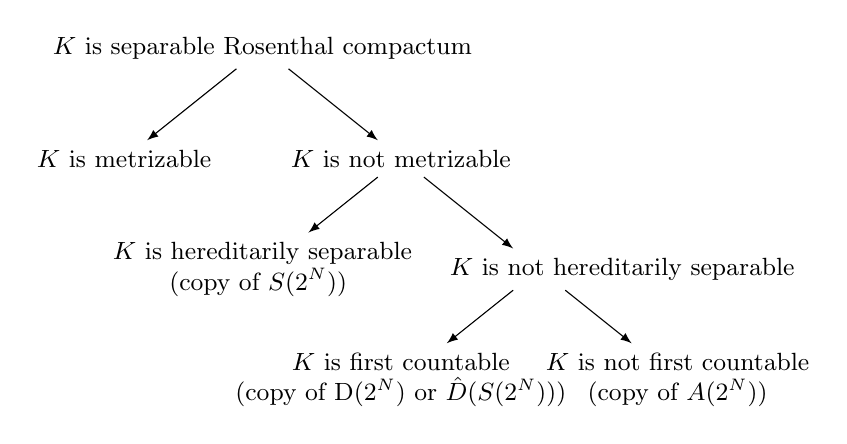
\begin{tikzpicture}[grow=down,
    sibling distance=10em,
    level distance=4em,
    edge from parent/.style={draw,-latex},
    every node/.style={font=\small,align=center}]

\node {$K$ is separable Rosenthal compactum}
    child {node {$K$ is metrizable}}
    child {node {$K$ is not metrizable}
    child {node {$K$ is hereditarily separable \\ (copy of $S(2^\mathbb{N})$) \hspace{2cm}}}
    child {node {\hspace{2cm} $K$ is not hereditarily separable}
    child {node {$K$ is first countable \\ (copy of $\mathrm{D}(2^\mathbb{N})$ or $\hat{D}(S(2^\mathbb{N}))$)}}
    child {node {$K$ is not first countable \\ (copy of $A(2^\mathbb{N})$)}}}};
\end{tikzpicture}
    \caption{Classification of separable Rosenthal compacta.}
    \label{fig:separable_compacta}
\end{figure}

Todorčević's Trichotomy suggests that in order to distinguish the classes $\NIP_i$, the examples in \ref{exa:Rosenthal-compacta} are essential.
The following examples show that the levels $\NIP_i$ ($i=1,2,3$) may be distinguished by the topological complexity of deep computations.

\begin{example}\label{exa:NIP-levels}
\hfill
\begin{enumerate}
    \item Let $(L,\mathcal{P},\Gamma)$ be the computation of square root (example \ref{exa:square-roots-compute} with $\Delta=\Gamma$).
    We saw that $\overline{\tilde{\Delta}}=\tilde{\Delta}\cup\{\tilde{f}\}\subseteq \mathrm{B}_1(\mathcal{L},\mathcal{L})$.
    This corresponds to the Alexandroff compactification of a countable discrete set, which is metrizable. Hence, $\Delta$ is $\NIP_3$ but it is not stable, in the sense that $\overline{\tilde{\Delta}}\not\subseteq \mathrm{C}(\mathcal{L},\mathcal{L})$.

    \item Let $(L,\mathcal{P},\Gamma)$ be the finite precision threshold classifiers (Section~\ref{sec:Cantor-classifiers}) with $\Delta=\{\phi_w:w\in 2^{<\mathbb{N}}\}\cup\{\mathbf{0^\infty},\mathbf{1^\infty}\}$.
    We saw that $\overline{\Delta}$ is homeomorphic to the Split Cantor space $S(2^\mathbb{N})$ (Example \ref{exa:Rosenthal-compacta}-(3)), which is hereditarily separable but not metrizable.
    Hence, $\Delta$ is $\NIP_2$ but not $\NIP_3$.

    \item Let $(L,\mathcal{P},\Gamma)$ be the CCS given by $L=2^{\mathbb{N}}$, $\mathcal{P}=\{P_n:n\in\mathbb{N}\}$ and $\Gamma$ is the semigroup generated by $\Delta=\{\gamma_t:t\in 2^{<\mathbb{N}}\}$, where $P_n\colon 2^\mathbb{N}\to\{0,1\}$ is the projection map $P_n(x)=x(n)$ and $\gamma_t\colon L\to L$ is given by
    \[
	\gamma_t(x)=\begin{cases}
        0^\infty, & \text{if }x<_{\text{lex}}t^\frown0^\infty;\\
        (01)^\infty, & \text{if }t^\frown0^\infty\leq_{\text{lex}} x \leq_{\text{lex}} t^\frown1^\infty;\\
        1^\infty, & \text{if }t^\frown1^\infty<_{\text{lex}}x.
    \end{cases}
    \]
    where $(01)^\infty$ denotes the sequence of alternating bits: $010101\cdots$. 
    As in the other examples, it is not difficult to see that $(L,\mathcal{P},\Gamma)$ satisfies the Extensibility Axiom.
    For example, the condition $t^\frown0^\infty\leq_{\text{lex}} x \leq_{\text{lex}} t^\frown1^\infty$ is equivalent to $x$ extending $t$.
    Observe that the set of deep computations is homeomorphic to $\hat{D}(S(2^{\mathbb{N}}))$ (see Example~\ref{exa:Rosenthal-compacta}-(5)).
    Hence, $\Delta$  is $\NIP_1$ but not $\NIP_2$.

    \item Let $(L,\mathcal{P},\Gamma)$ be the finite precision prefix test (Section~\ref{sec:prefix-test}) with $\Delta=\{\psi_w:w\in 2^{<\mathbb{N}}\}$.
    We saw that $\overline{\tilde{\Delta}}$ is homeomorphic to the Extended Alexandroff compactification $\hat{A}(2^\mathbb{N})$ (Example \ref{exa:Rosenthal-compacta}-(3)), which is separable but not first countable.
    Hence, $\Delta$ is NIP but not $\NIP_1$.
\end{enumerate}
\end{example}

The definitions provided here for $\NIP_i$ ($i=1,2,3$) are topological.
This raises the following question:

\begin{question}
    Is there a non-topological characterization for $\NIP_i$, $i=1,2,3$?
\end{question}

\subsection{The Argyros-Dodos-Kanellopoulos heptachotomy, and approximability of deep computation by minimal classes}\label{sec:heptachotomy}

In the three separable cases given in \ref{exa:Rosenthal-compacta}, namely, $\hat{A}(2^\mathbb{N})$, $S(2^\mathbb{N})$ and $\hat{D}(S(2^\mathbb{N}))$, the countable dense subsets are indexed by the binary tree $2^{<\mathbb{N}}$.
This choice of index is useful because our emphasis is computational.
Real numbers can be represented as infinite binary sequences, i.e., infinite branches of the binary tree $2^{\mathbb{N}}$, and
we approximate real numbers with elements in $2^{<\mathbb{N}}$, i.e., finite bitstrings.

\begin{definition}
    Let $X$ be a Polish space.

    \begin{enumerate}
        \item If $I$ is countable and $\{f_i:i\in I\}\subseteq\mathbb{R}^X$, $\{g_i:i\in I\}\subseteq\mathbb{R}^X$ are two pointwise families by $I$, we say that $\{f_i:i\in\ I\}$ and $\{g_i:i\in I\}$ are \emph{equivalent} if and only if the map $f_i\mapsto g_i$ is extended to a homeomorphism from $\overline{\{f_i:i\in I\}}$ to $\overline{\{g_i:i\in I\}}$.
        \item If $\{f_t:t\in 2^{<\mathbb{N}}\}$ is a pointwise bounded family, we say that $\{f_t:t\in 2^{<\mathbb{N}}\}$ is \emph{minimal} if and only if for every dyadic subtree $\{s_t:t\in 2^{<\mathbb{N}}\}$ of $2^{<\mathbb{N}}$, $\{f_{s_t}:t\in 2^{<\mathbb{N}}\}$ is equivalent to $\{f_t:t\in 2^{<\mathbb{N}}\}$.
    \end{enumerate}
\end{definition}

One of the main results in \cite{argyros2008rosenthal} is that, up to equivalence, there are seven minimal families of Rosenthal compacta and that for every relatively compact $\{f_t:t\in 2^{<\mathbb{N}}\}\subseteq \mathrm{B}_1(X)$ there is a dyadic subtree $\{s_t:t\in 2^{<\mathbb{N}}\}$ such that $\{f_{s_t}:t\in 2^{<\mathbb{N}}\}$ is equivalent to one of the minimal families.
We shall describe the seven minimal families next.
We follow the same notation as in \cite{argyros2008rosenthal}.
For any node $t\in 2^{<\mathbb{N}}$, we denote by $t^\frown 0^{\infty}$ ($t^\frown 1^{\infty}$) the infinite binary sequence starting with $t$ and continuing with all $0$'s (respectively, all $1$'s).
Fix a regular dyadic subtree $R=\{s_t:t\in 2^{<\mathbb{N}}\}$ of $2^{<\mathbb{N}}$ (i.e., a dyadic subtree such that every level of $R$ is contained in a level of $2^{<\mathbb{N}}$) with the property that for all $s,s'\in R$, we have $s^\frown 0^{\infty}\neq s'^\frown 0^\infty$ and $s^\frown 1^{\infty}\neq s'^\frown 1^\infty$.
Given $t\in 2^{<\mathbb{N}}$, let $v_t$ be the characteristic function of the set $\{x\in 2^\mathbb{N}:x \text{ extends } t\}$.
Let $<$ be the lexicographic order in $2^\mathbb{N}$.
Given $a\in 2^{\mathbb{N}}$, let $f^+_a\colon 2^{\mathbb{N}}\to\{0,1\}$ be the characteristic function of $\{x\in 2^{\mathbb{N}}:a\leq x\}$ and let $f^-_a\colon 2^{\mathbb{N}}\to\{0,1\}$ be the characteristic function of $\{x\in 2^{\mathbb{N}}:a>x\}$.
Given two maps $f,g\colon 2^{\mathbb{N}}\to\mathbb{R}$ we denote by $(f,g)\colon 2^{\mathbb{N}}\sqcup 2^{\mathbb{N}}\to\mathbb{R}$ the function which is $f$ on the first copy of $2^{\mathbb{N}}$ and $g$ on the second copy of $2^{\mathbb{N}}$.

\begin{enumerate}
    \item $D_1=\{\frac{1}{|t|+1}v_t:t\in 2^{<\mathbb{N}}\}$.
    This is discrete in $\overline{D_1}=A(2^{\mathbb{N}})$.
    \item $D_2=\{s_t^\frown 0^{\infty}:t\in 2^{<\mathbb{N}}\}$.
    This is discrete in $\overline{D_2}=2^{\leq N}$.
    \item $D_3=\{f^+_{s_t^\frown 0^\infty}:t\in 2^{<\mathbb{N}}\}$.
    This is discrete in $\overline{D_3}=S(2^{\mathbb{N}})$.
    \item $D_4=\{f^-_{s_t^\frown 1^\infty}:t\in 2^{<\mathbb{N}}\}$.
    This is discrete in $\overline{D_4}=S(2^{\mathbb{N}})$.
    \item $D_5=\{v_t:t\in 2^{<\mathbb{N}}\}$.
    This is discrete in $\overline{D_5}=\hat{A}(2^{\mathbb{N}})$.
    \item $D_6=\{(v_{s_t},s_t^\frown 0^\infty):t\in 2^{<\mathbb{N}}\}$.
    This is discrete in $\overline{D_6}=\hat{D}(2^{\mathbb{N}})$.
    \item $D_7=\{(v_{s_t},x^+_{s_t^\frown 0^\infty}):t\in 2^{<\mathbb{N}}\}$.
    This is discrete in $\overline{D_7}=\hat{D}(S(2^{\mathbb{N}}))$.
\end{enumerate}

\begin{theorem}[Heptachotomy of minimal families, Theorem 2 in \cite{argyros2008rosenthal}]
    Let $X$ be Polish.
    For every relatively compact $\{f_{t}:t\in 2^{<\mathbb{N}}\}\subseteq \mathrm{B}_1(X)$, there exists $i=1,2,\dots, 7$ and a regular dyadic subtree $\{s_t:t\in 2^{<\mathbb{N}}\}$ of $2^{<\mathbb{N}}$ such that $\{f_{s_t}:t\in 2^{<\mathbb{N}}\}$ is equivalent to $D_i$.
    Moreover, the families $D_i$ are minimal and mutually non-equivalent.
\end{theorem}

The implication of this result for deep computations is the following: 
for any countable set of computations $\Delta$ satisfying the NIP (for some CCS $(L,\mathcal{P},\Gamma)$), we can always find a countable discrete set of deep computations that approximates all the other deep computations.
For example: in the finite precision prefix test example (subsection \ref{sec:prefix-test}), the prefix test computations (family $D_5$) approximate all other deep computations.
However, note that this discrete set $D_i$ may not consist of continuous functions (i.e., they will not be computable in general).
For example, functions in $D_3$ are not continuous.
% /chapters/3-deep-computations/05-randomized.tex

\section{Monte Carlo computability}\label{sec:measure-theoretic-NIP}

In this section, we replace deterministic computability by probabilistic (`Monte Carlo') computability.
We do not assume that $\mathcal{P}$ is countable.
(The countability assumption on $\mathcal{P}$ played a crucial role in the proof of Theorem~\ref{thm:Generalized-BFT}, as it makes $\mathbb{R}^\mathcal{P}$ a Polish space.)
The main results of the section are Theorem~\ref{thm:NIP-Monte-Carlo}, which connects NIP and Monte Carlo computability, and~\ref{cor:Talagrand-stab-Monte-Carlo}, which connects Talagrand stability and Monte Carlo computability.

Fundamental in this section is a measure-theoretic version of Theorem~\ref{thm:Generalized-BFT}, namely, Theorem~\ref{thm:BFT-2F}.

\subsection{NIP and Monte Carlo computability of deep computations}

By Fact~\ref{baire}, for perfectly normal $X$, a function $f$ is in $\mathrm{B}_1(X,Y)$ if and only if $f^{-1}[U]$ is an $F_\sigma$ subset of $X$ for every open $U\subseteq Y$.
This motivates the following definition.

\begin{definition}\label{def:universal-measurability}
    Given a Hausdorff space $X$ and a measurable space $(Y,\Sigma)$, we say that $f\colon X\to Y$ is \emph{universally measurable} (with respect to $\Sigma$) if $f^{-1}(E)$ is $\mu$-measurable for every Radon measure $\mu$ on $X$ and every $E\in\Sigma$.
    When $Y=\mathbb{R}$, we will always take $\Sigma=\mathcal{B}(\mathbb{R})$, the Borel $\sigma$-algebra of $\mathbb{R}$.
\end{definition}

If $X$ is a compact (Hausdorff) space, then Radon measures on $X$ are finite, and hence, through renormalization, we can regard them as probability measures.
We thus have the following remark:

\begin{remark}\label{rem:probability}
If $X$ is compact, then a function $f\colon X\to\mathbb{R}$ is universally measurable if and only if $f^{-1}(U)$ is $\mu$-measurable for every Radon probability measure $\mu$ on $X$ and every open set $U\subseteq\mathbb{R}$.
\end{remark}

Intuitively, a function is universally measurable if it is ``measurable no matter which reasonable way you try to measure things on its domain".
The concept of universal measurability emerged from work of Kallianpur and Sazonov, in the late 1950's and 1960s --- with later developments by Blackwell, Darst and others --- building on earlier ideas of Gnedenko and Kolmogorov from the 1950s.
See~\cite[Chapters 1 and 2]{Pap:2002}.

\begin{notation}
    Following \cite{BFT_1978_PCompactBaire}, the collection of all universally measurable real-valued functions on $X$ will be denoted by $M_r(X)$.
    Given a fixed Radon measure $\mu$ on $X$, the collection of all $\mu$-measurable real-valued functions on $X$ will be denoted by $\mathscr{M}^0(X,\mu)$.
\end{notation}

In the context of deep computations, we are interested in transition maps of a state space $L\subseteq \mathbb{R}^\mathcal{P}$ into itself.
In the product space $\mathbb{R}^\mathcal{P}$, we have two natural $\sigma$-algebras: 
the Borel $\sigma$-algebra, i.e., the $\sigma$-algebra generated by open sets in $\mathbb{R}^\mathcal{P}$, and the cylinder $\sigma$-algebra (i.e., the $\sigma$-algebra generated by the sub-basic open sets in $\mathbb{R}^\mathcal{P}$, that is, the set $\pi_i^{-1}(U)$ with $U\subseteq \mathbb{R}$ open).
In general, the cylinder $\sigma$-algebra is strictly smaller; however, when $\mathcal{P}$ is countable, both $\sigma$-algebras coincide.
We will use the cylinder $\sigma$-algebra to define universally measurable maps $f\colon\mathbb{R}^\mathcal{P}\to\mathbb{R}^\mathcal{P}$.
The reason for this choice is the following characterization:

\begin{proposition}\label{prop:coordinated_univ_meas}
    Let $X$ be a Hausdorff space and $Y=\prod_{i\in I}Y_i$ be any product of measurable spaces $(Y_i,\Sigma_i)$ for $i\in I$.
    Let $\Sigma_Y$ be the cylinder $\sigma$-algebra generated by the measurable spaces $(Y_i,\Sigma_i)$.
    The following are equivalent for $f\colon X\to Y$:
    \begin{enumerate}[(i)]
        \item $f\colon X\to Y$ is universally measurable (with respect to $\Sigma_Y$).
        \item $\pi_i\circ f\colon X\to Y_i$ is universally measurable (with respect to $\Sigma_i$) for all $i\in I$.
    \end{enumerate}
\end{proposition}

\begin{proof}
    (i)$\Rightarrow$(ii) is clear since the projection maps $\pi_i$ are measurable and the composition of measurable functions is measurable.
    To prove (ii)$\Rightarrow$(i), note that if $C=\prod_{i\in I}C_i$ is a measurable cylinder and $J$ is the finite subset of $I$ such that $C_i\neq Y_i$ for $i\in J$, then, $f^{-1}(C)=\bigcap_{i\in J}(\pi_i\circ f)^{-1}(C_i)$ is universally measurable by assumption.
\end{proof}

The preceding proposition says that we can check measurability of a transition just by checking measurability feature by feature.
This is analogous to the Baire class 1 setting (see Proposition~\ref{prop:Baire-identifications}).

We saw in section \ref{sec:prelim} that, when the set $\mathcal{P}$ of predicates is countable, PAC-learning (or NIP) corresponds to relative compactness in the space of Baire class 1 functions (see Theorems~\ref{thm:BFT}, \ref{thm:BFT2}, \ref{thm:Generalized-BFT}).
The following result (which does not assume countability of $\mathcal{P}$) gives an analogous characterization of the NIP in terms of universal measurability:

\begin{theorem}
[Bourgain-Fremlin-Talagrand, Theorem 2F in \cite{BFT_1978_PCompactBaire}]\label{thm:BFT-2F}
    Let $X$ be a Hausdorff space and $A\subseteq \mathrm{C}(X)$ be pointwise bounded.
    The following are equivalent:
    \begin{enumerate}[(i)]
        \item $\overline{A}\subseteq M_r(X)$.
        \item For every compact $K\subseteq X$, $A\restriction_K$ satisfies the NIP.
        \item For every Radon measure $\mu$ on $X$, $A$ is relatively countably compact in $\mathscr{M}^0(X,\mu)$, i.e., every countable subset of $A$ has a limit point in $\mathscr{M}^0(X,\mu)$.
    \end{enumerate}
\end{theorem}

This result allows us to formalize the concept of a deep computation being \emph{Monte Carlo computable}, which we define below (Definition~\ref{def:universally-essentially-computable}).
To motivate the definition, let us first recall two facts:

\begin{enumerate}
    \item Littlewoood's second principle states that every Lebesgue measurable function is ``nearly continuous.''
The formal statement of this, which is Luzin's theorem, is that if $(X,\Sigma ,\mu )$ a Radon measure space and $Y$ is a second-countable topological space (e.g., $Y=\mathbb{R}^\mathcal{P}$ with $\mathcal{P}$ countable) equipped with the Borel $\sigma$-algebra, then any given $f:X\to Y$ is measurable if and only if for every $E\in\Sigma$ and every $\varepsilon>0$ there exists a closed $F\subseteq E$ such that the restriction $f\restriction_F$ is continuous and $\mu(E\backslash F) < \varepsilon$.

    \item Computability of deep computations is characterized in terms of continuous extensibility of computations.
    This is at the core of~\cite{alva2024approximability}.
\end{enumerate}

These two facts motivate the following definition:

\begin{definition}\label{def:universally-essentially-computable}
    Let $(L,\mathcal{P},\Gamma)$ be a CCS.
    We say that a transition $f\colon L\to L$ is \emph{universally Monte Carlo computable} if and only if there exists an extension $\tilde f:\colon\mathcal{L}_{\sh}\to \mathcal{L}_{\sh}$ of $f$ satisfying the following property: for every sizer $r_\bullet$ there is a sizer $s_\bullet$ such that the restriction $\tilde f\restriction_{\mathcal{L}[r_{\bullet}]}\colon\mathcal{L}[r_\bullet]\to\mathcal{L}[s_\bullet]$ is universally measurable, i.e., $\pi_P\circ \tilde f\restriction_{\mathcal{L}[r_{\bullet}]}\colon \mathcal{L}[r_\bullet]\to [-s_P,s_P]$ is $\mu$-measurable for every Radon probability measure $\mu$ on $\mathcal{L}[r_\bullet]$ and $P\in\mathcal{P}$.
\end{definition}

Note that, since $\mathcal{L}_{\sh}$ is compact, by remark~\ref{rem:probability}, in the context of Monte Carlo computability, we restrict our attention to Radon probability measures instead of general Radon measures.

\begin{theorem}\label{thm:NIP-Monte-Carlo}
    Let $(L,\mathcal{P},\Gamma)$ be a CCS satisfying the Extensibility Axiom.
    Let $R$ be an exhaustive collection of sizers.
    Let $\Delta\subseteq\Gamma$ be $R$-confined.
    If $\pi_P\circ\Delta\restriction_{L[r_\bullet]}$ satisfies the NIP for all $P\in\mathcal{P}$ and all $r_{\bullet}\in R$, then every deep computation in $\Delta$ is universally Monte Carlo computable.
\end{theorem}

\begin{proof}
    Fix $P\in\mathcal{P}$ and $r_\bullet\in R$.
    By the Extensibility Axiom, $\pi_P\circ\tilde\Delta\restriction_{\mathcal{L}[r_\bullet]}$ is a set of pointwise bounded continuous functions on the compact set $\mathcal{L}[r_\bullet]$.
    Since $\pi_P\circ\Delta\restriction_{L[r_\bullet]}$ has the NIP, so does $\pi_P\circ\tilde\Delta\restriction_{L[r_\bullet]}=\pi_P\circ\Delta\restriction_{\mathcal{L}[r_\bullet]}$, by Lemma \ref{lem:NIP-and-closure}.
    Let $f\in\overline{\Delta}$ be a deep computation;
     write $f$ as an ultralimit of computations in $\Delta$, say $f=\mathcal{U}\lim_i\gamma_i$ , and
    define an extension $\tilde{f}\colon\mathcal{L}_{\sh}\to \mathcal{L}_{\sh}$ of $f$ naturally by $\tilde{f}:=\mathcal{U}\lim_i\tilde{\gamma_i}$.
    Since, by hypothesis, $\Delta$ is $R$-confined, we have $f\colon L[r_\bullet]\to L[r_\bullet]$ and hence, $\tilde{f}\colon\mathcal{L}[r_\bullet]\to \mathcal{L}[r_\bullet]$.
    Now, by Theorem \ref{thm:BFT-2F}, we have $\overline{\pi_P\circ\tilde\Delta\restriction_{\mathcal{L}[r_\bullet]}}\subseteq M_r(\mathcal{L}[r_\bullet])$; therefore, $\pi_P \circ \tilde{f}\restriction_{\mathcal{L}[r_\bullet]}\in \overline{\pi_P\circ\tilde\Delta\restriction_{\mathcal{L}[r_\bullet]}}\subseteq M_r(\mathcal{L}[r_\bullet])$.
\end{proof}

\begin{question}
    Under the same assumptions of the preceding theorem, suppose that every deep computation of $\Delta$ is universally Monte Carlo computable.
    Must $\pi_P\circ\Delta\restriction_{L[r_\bullet]}$ have the NIP for all $P\in\mathcal{P}$ and all $r_{\bullet}\in R$?
\end{question}

\subsection{Talagrand stability and Monte Carlo computability of deep computations}

There is another notion closely related to NIP, introduced by Talagrand in \cite{talagrand1984pettis} while studying Pettis integration.
Suppose that $X$ is a compact Hausdorff space and $A\subseteq \mathbb{R}^X$.
Let $\mu$ be a Radon probability measure on $X$.
Given a $\mu$-measurable set $E\subseteq X$, a positive integer $k$ and real numbers $a<b$, let

\[
	D_k(A,E,a,b)=\bigcup_{f\in A}\{x\in E^{2k}:f(x_{2i})\leq a, \hspace{1mm} f(x_{2i+1})\geq b \hspace{1mm}{\text{ for all }i<k} \}.
\]

\begin{definition}\label{def:Talagrand-stable}
    We say that $A$ is \emph{Talagrand $\mu$-stable} if and only if for every $\mu$-measurable set $E\subseteq X$ of positive measure and for every $a<b$ there is $k\geq 1$ such that
    \[
    (\mu^{2k})^*(D_k(A,E,a,b))<(\mu(E))^{2k},
    \]
    where $\mu^*$ denotes the outer measure.
\end{definition}

Note that the reference to outer measure in Definition~\ref{def:Talagrand-stable} is necessary since $D_k(A,E,a,b)$ need not be measurable.
The inequality certainly holds when $A$ is a countable set of continuous (or $\mu$-measurable) functions.

\begin{remark}\label{rem:Talgrand-stability}
    Let $X$, $\mu$, $A\subseteq \mathbb{R}^X$, and $\subseteq X$ be as above. Then,
    \begin{enumerate}
        \item If $A\subseteq B\subseteq \mathbb{R}^X$, then \[D_k(A,E,a,b)\subseteq D_k(B,E,a,b).\]
        \item If $a<a'<b'<b$, then \[D_k(\overline{A},E,a,b)\subseteq D_k(A,E,a',b').\]

[\emph{Proof}: If $x\in D_k(\overline{A},E,a,b)$, then there is $f\in\overline{A}$ such that $f(x_{2i})\leq a<a'$ and $f(x_{2i+1})\geq b>b'$ for all $i<k$.
By definition of pointwise convergence topology, there exists $g\in A$ such that $g(x_{2i})<a'$ and $g(x_{2i+1})>b'$ for all $i<k$.
Hence, $x\in D_k(A,E,a',b')$.]

    \item Any subset of a $\mu$-stable set is $\mu$-stable. (This is immediate from (1).)

    \item If $A$ is stable, then $\overline{A}$ is $\mu$-stable. (This is immediate from (2).)
\end{enumerate}
\end{remark}

The main result of this section is that deep computations that are limit points of a Talagrand stable set of computations are Monte Carlo computable; this is Corollary~\ref{cor:Talagrand-stab-Monte-Carlo} below.
To prove it, we first show that the closure of a Talagrand $\mu$-stable set is $\mu$-measurable (lemma~\ref{lem:talagrand-stab-relcpct});
but first, we need the following useful characterization of measurable functions (compare with Fact \ref{baire}):

\begin{fact}[Lemma 413G in \cite{fremlin2003vol4}]\label{fact:meas-fns-charn}
    Suppose that $(X,\Sigma,\mu)$ is a measure space and let $\mathcal{K}\subseteq\Sigma$ be a collection of measurable sets satisfying the following conditions:
    \begin{itemize}
        \item $(X,\Sigma,\mu)$ is complete, i.e., for all $E\in\Sigma$ with $\mu(E)=0$ and $F\subseteq E$ we have $F\in\Sigma$.
        \item $(X,\Sigma,\mu)$ is semi-finite, i.e., for all $E\in\Sigma$ with $\mu(E)=\infty$ there exists $F\subseteq E$ such that $F\in\Sigma$ and $0<\mu(F)<\infty$.
        \item $(X,\Sigma,\mu)$ is saturated, i.e., $E\in\Sigma$ if and only if $E\cap F\in\Sigma$ for all $F\in\Sigma$ with $\mu(F)<\infty$.
        \item $(X,\Sigma,\mu)$ is inner regular with respect to $\mathcal{K}$, i.e., for all $E\in\Sigma$
        \[
	\mu(E)=\sup\{\mu(K):K\in\mathcal{K} \text{ and } K\subseteq E\}.
        \]
    \end{itemize}
    (In particular, if $X$ is compact Hausdorff, $\mathcal{K}$ is the collection of compact subsets of $X$, $\mu$ is a Radon probability measure on $X$, $\Sigma$ is the completion of the Borel $\sigma$-algebra by $\mu$, and all these conditions hold).
    Then, $f\colon X\to\mathbb{R}$ is measurable if and only if for every $K\in\mathcal{K}$ with $0<\mu(K)<\infty$ and $a<b$, either $\mu^*(P)<\mu(K)$ or $\mu^*(Q)<\mu(K)$, where $P=\{x\in K:f(x)\leq a\}$ and $Q=\{x\in K:f(x)\geq b\}$.
\end{fact}

The following technical lemma will be instrumental for proving Proposition~\ref{prop:Talagrand-implies-NIP}, which, in turn, will yield the main result of the subsection, namely Corollary~\ref{cor:Talagrand-stab-Monte-Carlo}

\begin{lemma}\label{lem:talagrand-stab-relcpct}
    If $A$ is Talagrand $\mu$-stable, then $\overline{A}$ is also Talagrand $\mu$-stable and $\overline{A}\subseteq\mathscr{M}^0(X,\mu)$.
\end{lemma}

\begin{proof}
    If $A$ is Talagrand $\mu$-stable, so is $\overline{A}$, by Remarks~\ref{rem:Talgrand-stability}.
    Suppose that $A$ is Talagrand $\mu$-stable to show that $\overline{A}\subseteq \mathscr{M}^0(X,\mu)$.
    Assume, for the sake of contradiction that there exists $f\in\overline{A}$ such that $f\notin \mathscr{M}^0(X,\mu)$.
    By Fact \ref{fact:meas-fns-charn}, there exists a $\mu$-measurable set $E$ of positive measure and $a<b$ such that $\mu^*(P)=\mu^*(Q)=\mu(E)$ where $P=\{x\in E: f(x)\leq a\}$ and $Q=\{x\in E: f(x)\geq b\}$.
    Then, for any $k\geq 1$: $(P\times Q)^k\subseteq D_k(\{f\},E,a,b)$, so $(\mu^{2k})^*(D_k(\{f\},E,a,b))=(\mu^*(P)\mu^*(Q))^k=(\mu(E))^{2k}$.
    Thus, the set $\{f\}$ is not $\mu$-stable. 
    However, $\{f\}\subseteq\overline{A}$ and we know (Remarks~\ref{rem:Talgrand-stability}) that a subset of a $\mu$-stable set must be $\mu$-stable,
    so we have a contradiction.
\end{proof}

\begin{definition}
We say that $A$ is \emph{universally Talagrand stable} if $A$ is Talagrand $\mu$-stable for every Radon probability measure $\mu$ on $X$.
\end{definition}

We first observe that universal Talagrand stability implies NIP:

\begin{proposition}\label{prop:Talagrand-implies-NIP}
    Let $X$ be a compact Hausdorff space and $A\subseteq \mathrm{C}(X)$ be pointwise bounded.
    If $A$ is universally Talagrand stable, then $A$ satisfies the NIP.
\end{proposition}

\begin{proof}
    Suppose that $A$ is universally Talagrand stable.
    By Theorem \ref{thm:BFT-2F}, it suffices to show that $A$ is relatively countably compact in $\mathscr{M}^0(X,\mu)$ for every Radon probability measure $\mu$ on $X$.
    Since, for any such $\mu$, $A$ is Talagrand $\mu$-stable, Lemma \ref{lem:talagrand-stab-relcpct} gives us $\overline{A}\subseteq\mathscr{M}^0(X,\mu)$.
    In particular, $A$ is relatively countably compact in $\mathscr{M}^0(X,\mu)$.
\end{proof}

\begin{corollary}
\label{cor:Talagrand-stab-Monte-Carlo}
    Let $(L,\mathcal{P},\Gamma)$ be a CCS satisfying the Extensibility Axiom.
If $\pi_P\circ\Delta\restriction_{L[r_\bullet]}$ is universally Talagrand stable for all $P\in\mathcal{P}$ and all sizers $r_{\bullet}$, then every deep computation is universally Monte Carlo computable.
\end{corollary}

\begin{proof}
    This follows directly from Proposition \ref{prop:Talagrand-implies-NIP} and Theorem~\ref{thm:NIP-Monte-Carlo}.
\end{proof}

In the context of deep computations, we have identified two ways to obtain Monte Carlo computability, namely, NIP/PAC and Talagrand stability.
It is natural to ask whether these two notions are equivalent. 
The following results show that, even in the simple case of countably many computations, this question is sensitive to the set-theoretic axioms. 
On the one hand, it is consistent (with respect to the standard ZFC axioms of set theory) that these two classes are the same:

\begin{theorem}[Talagrand, Theorem 9-3-1(a) in \cite{talagrand1984pettis}]\label{thm:NIP-implies-Talagrand-stab}
    Let $X$ be a compact Hausdorff space and $A\subseteq M_r(X)$ be countable and pointwise bounded.
    Assume that $[0,1]$ is not the union of $<\mathfrak{c}$ closed measure zero sets.
If $A$ satisfies the NIP, then $A$ is universally Talagrand stable.
\end{theorem}

(The assumption that $[0,1]$ is not the union of $<\mathfrak{c}$ closed measure zero sets is a consequence of, for example, the Continuum Hypothesis.)

On the other hand, the opposite is also consistent for the particular case of the Lebesgue measure:

\begin{theorem}[Fremlin, Shelah, \cite{fremlin1993pointwise}]
    It is consistent with the usual axioms of set theory that there exists a countable pointwise bounded set of Lebesgue measurable functions with the NIP which is not Talagrand stable with respect to Lebesgue measure.
\end{theorem}

Notice that the preceding two results apply to sets of measurable functions, a class of functions larger than the class of continuous functions.
However, by the Extensibility Axiom, finitary computations are continuous, i.e., if $A$ is a set of computations, then $A\subseteq \Cp(X)$.